\documentclass{article}
\usepackage{graphicx}
\usepackage{tikz}
\usepackage{amsmath}
\usepackage{amssymb}
\usepackage{amsmath}
\usepackage{amssymb}
\usepackage{stmaryrd}
\usepackage{mathpartir}
\usepackage{tikz}
\usepackage{amsthm}
\usepackage{footnote}
\usepackage[italian]{babel}
\makesavenoteenv{figure}
\usepackage{geometry}

\theoremstyle{plain}
\newtheorem{thm}{Theorem}[section]
\newtheorem{cor}[thm]{Corollary}
\newtheorem{lem}[thm]{Lemma}
\newtheorem{prop}[thm]{Proposition}
\theoremstyle{definition}
\newtheorem{defi}[thm]{Definition}
\newtheorem{exa}[thm]{Example}
\theoremstyle{plain}
\setlength{\emergencystretch}{2em}
\usetikzlibrary{arrows.meta, positioning, calc, shapes.geometric}

\def \config#1{\langle #1 \rangle}
\newcommand{\mi}[1]{\mathit{#1}}
\newcommand{\ms}[1]{\mathsf{#1}}
\newcommand{\rules}[1]{\textsc{#1}}
\newcommand \tuple[2]{ #1 \vdash #2}
\newcommand{\il}[1]{{\color{green}#1}}
\newcommand{\red}[1]{\textcolor{red}{#1}}
\newcommand{\kw}[1]{\textcolor{black}{\textbf{#1}}}
\newcommand{\filename}[1]{\urlstyle{tt}\url{#1}}
\newcommand{\block}{\mathit{block}} 
\newcommand{\p}{\rho}
\newcommand{\nxt}{next}
\newcommand{\cnxt}{cnext} 
\newcommand{\s}{\pi}
\newcommand{\h}{h}
\newcommand{\init}{init}
\newcommand{\final}{final}
\newcommand{\cons}{\!:\!}
\newcommand{\flow}{\mathit{flow}}
\newcommand{\iflow}{\mathit{flow}^{-1}}
\newcommand{\entry}{\mathit{entry}}
\newcommand{\exit}{\mathit{exit}}
\newcommand{\true}{\mathsf{true}}
\newcommand{\false}{\mathsf{false}}
\newcommand{\context}{\mathsf{ctx}}
\newcommand{\cont}{\mathsf{cont}}
\newcommand{\nul}{[\:]}
\newcommand{\emptystate}{\epsilon}
\newcommand{\emptystore}{\epsilon}
\newcommand{\rlh}{\rightleftharpoons}
\newcommand{\lh}{\leftharpoondown}
\newcommand{\rh}{\rightharpoonup}
\newcommand{\id}{\epsilon}
\newcommand{\edge}{\longrightarrow}
\newcommand{\iedge}{\stackrel{\mbox{\tiny -1}}{\longrightarrow}}

\def\defemb#1#2{\expandafter\def\csname #1\endcsname
                              {\relax\ifmmode #2\else\hbox{$#2$}\fi}}
\defemb{cA}{\mathcal{A}}
\defemb{cB}{\mathcal{B}}
\defemb{cC}{\mathcal{C}}
\defemb{cD}{\mathcal{D}}
\defemb{cE}{\mathcal{E}}
\defemb{cF}{\mathcal{F}}
\defemb{cG}{\mathcal{G}}
\defemb{cH}{\mathcal{H}}
\defemb{cI}{\mathcal{I}}
\defemb{cJ}{\mathcal{J}}
\defemb{cL}{\mathcal{L}}
\defemb{cM}{\mathcal{M}}
\defemb{cN}{\mathcal{N}}
\defemb{cO}{\mathcal{O}}
\defemb{cP}{\mathcal{P}}
\defemb{cQ}{\mathcal{Q}}
\defemb{cR}{\mathcal{R}}
\defemb{cS}{\mathcal{S}}
\defemb{cT}{\mathcal{T}}
\defemb{cU}{\mathcal{U}}
\defemb{cV}{\mathcal{V}}
\defemb{cW}{\mathcal{W}}
\defemb{cX}{\mathcal{X}}
\defemb{cZ}{\mathcal{Z}}

\geometry{top=3.8cm, bottom=4.5cm, left=4.3cm, right=4.3cm}
\begin{document}

\newgeometry{top=2cm, textwidth=450pt, left=1.1in}
\begin{titlepage}
\begin{center}


\includegraphics[width=0.25\linewidth]{logo_unibo.png}\vspace{0.7cm}\\

{{\Large{\textsc{Alma Mater Studiorum $\cdot$ Universit\`a di
Bologna}}}} \rule[0.1cm]{15.8cm}{0.1mm}
\rule[0.5cm]{15.8cm}{0.6mm}

{\small{\bf Dipartimento di Informatica --- Scienza e Ingegneria\\
Corso di Laurea Triennale in Informatica}}
\end{center}

\vspace{15mm}
\begin{center}
{\LARGE{\bf Debugger step-by-step per il linguaggio di programmazione reversibile Janus}}\\
\vspace{3mm}

\vspace{19mm}

%{\large{\bf Tesi di Laurea in ''Settore Scientifico di Riferimento'' %\textit{(Opzionale)}}}
\end{center}

\vspace{30mm}
\par
\noindent
\begin{minipage}[t]{0.50\textwidth}

{\large{\bf Relatore:\\
Prof.\\
Ivan Lanese}} \\[5mm]

\end{minipage}
\hfill
\begin{minipage}[t]{0.47\textwidth}\raggedleft

{\large{\bf Presentata da:\\
Francesco Galavotti}}
\end{minipage}

\vspace{10mm}
\begin{center}

{\large{\bf Sessione 16 Dicembre 2026 \\}}
{\large{\bf Anno Accademico 2025/2026\\}}
\end{center}
\end{titlepage}

\restoregeometry

%\title{Debugger step-by-step per il linguaggio di programmazione reversibile Janus}
%\author{Francesco Galavotti}
%\date{16.12.2026}
%\maketitle

\section{Introduzione}\label{intro}

Un sistema computazione reversibile è caratterizzato dall'avere in qualunque momento uno stato di computazione precedente e uno stato di computazione successivo a quello corrente, e di conseguenza puo spostarsi deterministicamente in una direzione o l'altra. L'obiettivo della programmazione reversibile è quello di ridurre la dissipazione del calore al livello fisico della computazione. Vuole risolvere il problema posto da Landauer~\cite{landauerIrreversibilityHeatGeneration1961}, che ha dimostrato come un processo computazionale dove lo stato precedente non è univocamente determinato deve dissipare un quantitativo minimo di calore, quindi ogni volta che un singolo bit di informazione viene scartato in una computazione irreversibile. La programmazione reversibile si basa invece sul lavoro di Bennett~\cite{Bennett}, che ha dimostrato come, a livello teorico, una computazione reversibile in cui nessuna informazione è scartata, può essere eseguita con meno dissipazione di calore di una irreversibile.
\medskip

Oltre al livello fisico legato allo sviluppo di circuiti reversibili, per riuscire a riutilizzare il maggior quantitativo di energia (ed evitare la dissipazione del calore) all'interno di sistemi reversibili, è necessario prendere in considerazione anche una logica reversibile al livello del software. Il principale linguaggio di programmazione reversibile è Janus, questo è il primo del suo genere, ogni programma, procedura (funzione), costrutto o operazione è invertibile ed eseguibile in entrambe le direzioni. Questo significa che se un programma a cui assegnamo uno stato iniziale delle variabili \emph{x} arriva a fine esecuzione ad ottenere lo stato finale \emph{x'}, allora è possibile eseguire l'\emph{inverso} del programma e partire dallo stato \emph{x'} per ottenere, a fine computazione, lo stato \emph{x}. La stessa logica si applica anche alle procedure e grazie alla struttura del linguaggio l'inversione non richiede la scrittura manuale della procedura inversa.
\centerline{\emph{forward}: call $pgm$ $\sim$ uncall $pgm^{-1}$}
\centerline{\emph{backward}: uncall $pgm$ $\sim$ call $pgm^{-1}$}
L'inversione di programmi o procedure è un processo deterministico ed è strettamente legato alla reversibilità della computazione. Infatti l'esecuzione in avanti di un programma equivale all'esecuzione all'indietro dell'inverso dello stesso, e l'esecuzione all'indietro di un programma equivale all'esecuzione in avanti dell'inverso dello stesso ~\cite{JanusSem}.
\medskip

Sebbene la semantica illustrata nell'articolo originale di presentazione del linguaggio sia costruita in maniera "big-step", altre ricerche~\cite{LV26} hanno poi presentato una più recente semantica "small-step" e reversibile utile per permettere lo sviluppo di nuove funzionalità per il linguaggio. La natura bidirezionale di questa semantica apre nuove possibilità nell'analisi e nel controllo dell'esecuzione del codice. E' grazie a questa semantica, infatti, che è stato costruito il debugger presentato in questo documento, definito step-by-step e reversibile perchè ha la capacità di andare avanti e indietro a singoli passi durante l'esecuzione del programma. Rende quindi la fase di debugging del programmatore più semplice, in quanto è possibile analizzare lo stato di memoria ad ogni singolo step e si puo avanzare o indietreggiare a piacimento tra le operazioni e i breakpoint durante l'esecuzione. Di seguito andremo ad analizzare il funzionamento con le relative possibilità che il debugger offre e la struttura del codice con le relative scelte architetturali fatte, in modo da fornire al lettore la completa capacità d'uso e di manutenzione del debugger, nonché una panoramica dei possibili sviluppi futuri.

\section{Il linguaggio di programmazione reversibile Janus}

Nel seguente capitolo vogliamo introdurre il linguaggio di programmazione Janus, i suoi costrutti e le sue peculiarità. E' un linguaggio reversibile, questo significa che ogni programma, procedura o operazione può essere eseguita in entrambe le direzioni, avanti (forward) e indietro (backward). Ci atterremo alla struttura presentata nel documento originale di presentazione del linguaggio~\cite{YOKOYAMA201071,LoopSem,JanusSem}.

\begin{figure}[h]
\small
\begin{center}
$
\begin{array}{rcl@{~~~~~~}rcl@{ }}
\mi{p} & ::= & \mi{d}^{*} ~(\ms{procedure} ~id~s)^{+} & \\
\mi{d} & ::= & x  \mid x[c]  &\\
\mi{s} & ::= & x \oplus = e \, \mid \, x[e]\oplus=e \, \mid \ms{if}~e ~\ms{then} ~s~\ms{else}~s~\ms{fi}~e \\
& \mid & \ms{from}~e~\ms{do}~s~\ms{loop}~s~\ms{until}~e \,
\mid \ms{call}~id \, \mid \, \ms{uncall}~id\mid \, \ms{skip} \, \mid \, s~s\\
\mi{e} & ::= & c \mid x  \mid x[e] \mid e \odot e \\
\oplus & ::= &  + \mid - \mid \hat{~}\\
\mi{c} & ::= & - 2147483648\mid \dots \mid 0 \mid \dots \mid 2147483647 \\
\odot & ::= & \oplus \mid \mbox{\tt *} \mid \mbox{\tt /} \mid \mbox{\tt \%} \mid \mbox{\tt \&} \mid \mbox{\tt \&\&} \mid \mbox{\tt ||} \mid \mbox{\tt |}
\mid \mbox{\tt <} \mid \mbox{\tt >} \mid \mbox{\tt =} \mid \mbox{\tt !=} \mid \mbox{\tt <=} \mid \mbox{\tt >=} &
\end{array}
$
\end{center}
\caption{Sintassi di Janus} \label{syntax}
\end{figure}

\begin{figure}[!h]
    \centering
    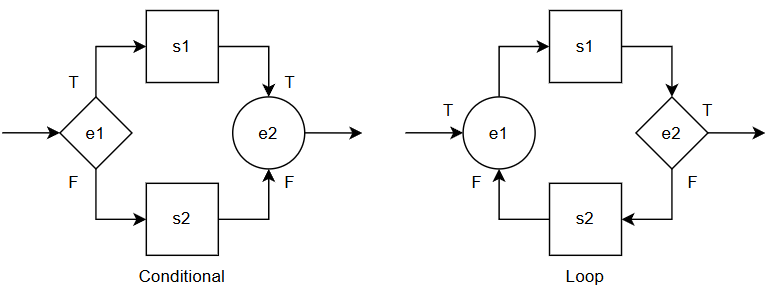
\includegraphics[width=0.9\textwidth]{pictures/condandloop.png}
    \caption{Diagrammi del condizionale e del loop}
    \label{fig:condandloop}
\end{figure}

In Figura~\ref{syntax} è presentata la sintassi di Janus. Un programma comincia con una serie di dichiarazioni di variabili e array, i valori supportati sono solamente gli interi e tutte le variabili e posizioni negli array partono a inizio programma col valore zero. Seguono poi, le dichiarazioni delle procedure, ognuna di queste introdotta con la keyword "procedure" e identificata da un nome (id) e una serie di statements. Le procedure non hanno né parametri né variabili locali. Gli statement rappresentano le operazioni e i costrutti che il programmatore può utilizzare mentre scrive codice Janus, ognuno di questi è reversibile.

Lo statement di assegnamento prende la forma ``$x \oplus = e$'' (o ``$x[e_1] \oplus = e_2$'' per gli assegnamenti ad array), ed equivale a $x = x \oplus e$ (\ $x[e_1] = x[e_1]\oplus e_2$), dove $\oplus$ rappresenta un operatore tra più, meno e lo xor bitwise. Janus richiede che la variabile sul lato sinistro dell'operazione, $x$, non compaia nell'espressione $e$ (nel caso di array non deve comparire né in $e_1$ né in $e_2$). Gli assegnamenti vanno quindi a modificare il valore delle variabili senza sovrascriverlo, questo per garantire la reversibilità evitando di scartare informazioni (vedi Introduzione, capitolo~\ref{intro}).

Janus include anche un'istruzione di scambio che prende la forma ``$e <=> e$'', dove $e ::= x \mid x[e]$, e la sua funzione è quella di scambiare il valore di due variabili (o elementi di array), anche qui Janus richiede che la variabile sul lato sinistro dell'operazione, $x$, non compaia nell'espressione $e$. Questa istruzione è zucchero sintattico che abbrevia la sequenza di statement: $x1 \mathbin{\text{\^{}}}= x2$ ; $x2 \mathbin{\text{\^{}}}= x1$ ; $x1 \mathbin{\text{\^{}}}= x2$.

Lo statement di condizione prende la forma: ``$\ms{if}~e_1~\ms{then}~s_1~\ms{else}~s_2~\ms{fi}~e_2$.'', le due condizioni $e_1$ e $e_2$ sono chiamate rispettivamente \emph{test} e \emph{assertion}. Se il valore del test è \emph{true} allora viene eseguito il blocco di statement \emph{s1}, altrimenti viene eseguito il blocco \emph{s2}, perchè la condizione sia valida il valore dell'assertion deve essere lo stesso del test, questo serve a garantire la reversibilità in quanto un'esecuzione backward del programma riesce ad entrare nel path giusto del condizionale.

Lo statement del ciclo prende la forma: ``$\ms{from}~e_1~\ms{do}~s_1~\ms{loop}~s_2~\ms{until}~e_2$''. Qui, $e_1$ prende il nome di assertion e $e_2$ prende il nome di test, perchè il ciclo sia valido la prima valutazione dell'assertion deve avere come risultato \emph{true}, quindi gli statement in $s_1$ vengono eseguiti. Ora viene valutata la seconda condizione, il test $e_2$, se questa corrisponde al valore \emph{true} allora il loop termina, altrimenti vengono eseguiti gli statement all'interno di $s_2$. In quest'ultimo caso il controllo ritorna poi all'assertion $e_1$ che deve però avere come valore \emph{false}, e viene eseguito nuovamente $s_1$. Il ciclo si ripete finche il test $e_2$ non corrisponde a \emph{true}.

Gli statement di chiamata a procedura sono due e prendono le forme: ``$\ms{call}~\mathit{id}$'' per eseguire la procedura nel modo in cui è stata scritta (forward) e ``$\ms{uncall}~\mathit{id}$'' per eseguire la versione inversa della stessa procedura (backward).

In Figura~\ref{syntax} è anche illustrato l'intervallo di interi che le variabili possono assumere come valore e che possono essere usati come costante all'interno di espressioni, inoltre sono mostrati anche gli operatori aritmetici (+, -, *, /, \%), relazionali ($<$, $>$, =, !=, $<$=, $>$=), bitwise (\&, $|$, \textasciicircum{}) e logici (\&\&, $|$$|$) utilizzabili nelle espressioni.
\bigskip

\begin{figure}[h]
\small
\begin{center}
$
\begin{array}{rcl@{~~~~~~}rcl@{ }}
\mathcal{I}_{op}\llbracket + \rrbracket ::= - \hspace{1,5cm} 
\mathcal{I}_{op}\llbracket - \rrbracket & ::= & + \hspace{1,5cm}
\mathcal{I}_{op}\llbracket \hat{~} \rrbracket ::= \hat{~} \\
\mathcal{I}\llbracket x\oplus= e \rrbracket & ::= & x~\mathcal{I}_{op}\llbracket \oplus \rrbracket= e \\
\mathcal{I}\llbracket  x[e_1]\oplus=e_2 \rrbracket & ::= & x[e_1]~\mathcal{I}_{op}\llbracket \oplus \rrbracket= e_2 \\
\mathcal{I}\llbracket \ms{if}~e_1 ~\ms{then} ~s_1~\ms{else}~s_2~\ms{fi}~e_2 \rrbracket & ::= & \ms{if}~e_2 ~\ms{then} ~\mathcal{I}\llbracket s_1 \rrbracket~\ms{else}~\mathcal{I}\llbracket s_2 \rrbracket~\ms{fi}~e_1 \\
\mathcal{I}\llbracket \ms{from}~e_1~\ms{do}~s_1~\ms{loop}~s_2~\ms{until}~e_2 \rrbracket & ::= & \ms{from}~e_2~\ms{do}~\mathcal{I}\llbracket s_1 \rrbracket~\ms{loop}~\mathcal{I}\llbracket s_2 \rrbracket~\ms{until}~e_1 \\		
\mathcal{I}\llbracket \ms{call}~id \rrbracket & ::= & \ms{uncall}~id \\
\mathcal{I}\llbracket \ms{uncall}~id \rrbracket & ::= &   \ms{call}~id \\
\mathcal{I}\llbracket \ms{skip} \rrbracket & ::= & \ms{skip} \\
\mathcal{I}\llbracket s_1~s_2 \rrbracket & ::= & \mathcal{I}\llbracket s_2 \rrbracket ~ \mathcal{I}\llbracket s_1 \rrbracket \\
\mathcal{I}\llbracket \ms{procedure}~id~s \rrbracket & ::= & \ms{procedure} ~id^{-1}~\mathcal{I}\llbracket s \rrbracket \\
%\mathcal{I}\llbracket \ms{send}~x~ch \rrbracket & ::= & \ms{rec}~x~ch \\
%\mathcal{I}\llbracket \ms{rec}~x~ch \rrbracket & ::= & \ms{send}~x~ch \\
\end{array}
$
\end{center}
\caption{Funzione di inversione degli statement Janus} \label{fig:inverter}
\end{figure}

\section{Semantica reversibile per Janus}
\label{sec:LV26}
Visto che la semantica presentata nel paper originale di Janus prende la forma cosiddetta "big-step", che è inadatta alla reversibilità dei singoli step, introduciamo ora la semantica reversibile e "small-step" effettivamente utilizzata nell'implementazione del debugger \cite{LV26}.
\bigskip

Questa semantica si basa sull'utilizzo di un \emph{program counter} che punta al prossimo statement da eseguire. E' inoltre divisa in una relazione di transizione forward che gestisce l'esecuzione in avanti, e una relazione di transizione backward che gestisce quella all'indietro, e quindi può essere utilizzata per annullare i passi fatti dalla relazione forward.

\begin{figure}[h]
\small
%		\begin{center}
\begin{mathpar}
\inferrule*[left=Con] 
{ ~	} 
{ \tuple{\sigma}{c} \Downarrow  \llbracket c \rrbracket }     
\and
\inferrule*[left=Var] 
{ ~	} 
{ \tuple{\sigma}{ x} \Downarrow  \sigma(x)}      
\and
\inferrule*[left=Arr] 
{  \tuple{\sigma}{ e} \Downarrow v } 
{ \tuple{\sigma}{ x[e]} \Downarrow  \sigma(x[v]) }     
\and
\inferrule*[left=Bop] 
{ \tuple{\sigma}{ e_1} \Downarrow	 v_1 \\
\tuple{\sigma}{ e_2} \Downarrow	 v_2\\
\llbracket \odot \rrbracket(v_1,v_2) = v
} 
{ \tuple{\sigma}{ e_1 \odot e_2} \Downarrow  v }
\end{mathpar}
\caption{Semantica delle espressioni} \label{fig:exp}
%\end{center}
\end{figure}

Nel caso della valutazione delle espressioni, la semantica reversibile riutilizza le regole appartenenti alla semantica big-step originale, mostrate in Figura~\ref{fig:exp}, senza modificarle. Una regola di forma $\tuple{\sigma}{e} \Downarrow  v$ indica la valutazione dell'espressione $e$ ad uno stato \emph{store} $\sigma$ dello store globale delle variabili, che genera il valore $v$. Uno \emph{store} $\sigma$ è una funzione che associa nomi di variabile e nomi di array con indice a valori. Rappresentiamo con $\sigma[x \mapsto v]$ l'aggiornamento di $\sigma$ che assegna il valore $v$ alla variabile $x$. Allo stesso modo, $\sigma[x[v] \mapsto v']$ rappresenta l'aggiornamento di $\sigma$ che assegna il valore $v'$ all'array $x[v]$. Lo store $\sigma$ è definito (con valore zero se non diversamente inizializzato esplicitamente) per tutte le variabili usate nel programma. Con $\emptystore$ rappresentiamo uno store vuoto, che quindi associa zero ad ogni variabile (all'inizio del programma lo store è $\emptystore$). Qui, $\llbracket \_ \rrbracket$ indica una funzione che calcola un risultato tra valori interi facendo uso di un operatore.

Le regole in Figura~\ref{fig:exp} illustrano, quindi, come le espressioni sono valutate. Variabili e nomi di array con indice restituiscono il valore presente nello store, gli interi costanti restituiscono il loro valore e una operazione tra due espressioni le valuta entrambe e restituisce il risultato dell'operazione, eseguita tra i valori di queste.
\bigskip

Per gestire il controllo del program counter questa semantica introduce una struttura chiamata Control-Flow Graph (CFG), per fare ciò, il programma viene diviso in \emph{blocchi}, (ad esempio assegnamenti, condizioni, chiamate a procedura etc...), ognuno di questi rappresenta una istruzione elementare del programma ed è identificato da una label (etichetta), ogni label è unica nel programma. Inoltre, ad ogni procedura vengono aggiunti due blocchi, uno di \emph{start} ed uno di \emph{stop}, rispettivamente all'inizio e alla fine della procedura. In Figura~\ref{fig:labeled-syntax} è illustrata l'estensione della sintassi originale, prevista da questa semantica reversibile. La Figura~\ref{fig:programsum}, invece, mostra un programma Janus etichettato, MCM che calcola il minimo comune multiplo tra due numeri \emph{x} e \emph{y} e funge da esempio.

\begin{figure}[h]
\small
\begin{center}
$
\begin{array}{rcl@{~~~~~~}rcl@{ }}
%\mi{p} & ::= & s ~(\ms{procedure} ~id~s)^{*} & \\
%\mi{d} & ::= & x  \mid x[c]  &\\
\mi{s} & ::= & \red{[}x \oplus = e\red{]^\ell} \, \mid \, 
\red{[}x[e]\oplus=e\red{]^\ell} \,
\mid 
\ms{if}~\red{[}e\red{]^\ell} ~\ms{then} ~s~\ms{else}~s~\ms{fi}~
\red{[}e\red{]^\ell} \\
& \mid & 
\ms{from}~\red{[}e\red{]^\ell}~\ms{do}~s~\ms{loop}~s~\ms{until}~\red{[}e\red{]^\ell} \,
\mid 
\red{[} \ms{call}~id\red{]^\ell} \, \mid \, 
\red{[} \ms{uncall}~id\red{]^\ell} \mid \, 
\red{[} \ms{skip}\red{]^\ell} \, \mid \, s~s\\
& \mid & \red{[\ms{start}]^\ell} \, \mid \, \red{[\ms{stop}]^\ell} %\\
%& \mid & \ms{send}~x~ch \, \mid \, 
%\ms{rec}~x~ch \\
%\mi{e} & ::= & c \mid x  \mid x[e] \mid e \odot e \\
%\mi{c} & ::= & - 2147483648\mid \dots \mid 0 \mid \dots \mid 2147483647 \\
%\oplus & ::= &  + \mid - \mid \hat{~}\\
%\odot & ::= & \oplus \, \mid \, * \, \mid\, / \, \mid\,  \% \, \mid \, \& \, \mid\, \&\& \, \mid\,  \|  \, \mid\,  ''~|~'' \, 
%\mid \, < \, \mid \, > \, \mid \, = \, \mid \, ! = \, \mid \, <= \, \mid\, >= &
\end{array}
$
\end{center}
\caption{Estensione della sintassi del linguaggio ($\mi{e}$ e $\oplus$ sono definiti come in Figura~\ref{syntax})} \label{fig:labeled-syntax}
\end{figure}

\begin{figure}[h]
    \centering
    \begin{minipage}{0.95\textwidth}
        \ttfamily 
        % --- Left Column ---
        \begin{minipage}[t]{0.28\textwidth}
            x \\{}
            y \\{}
            i \\{}
            mcm \\{}
            \\{}
            \kw{procedure} main \\{}
            \hspace*{1em}[\kw{start}]$^1$ \\ \protect
            \hspace*{1em}[x += 5]$^2$ \\{}
            \hspace*{1em}[y += 3]$^3$ \\{}
            \hspace*{1em}{[\kw{call} MCM]}$^4$ \\
            \hspace*{1em}{[\kw{stop}]}$^5$
        \end{minipage}
        \hfill 
        % --- Right Column ---
        \begin{minipage}[t]{0.68\textwidth}
            \kw{procedure} MCM \\
            \hspace*{1em} [\kw{start}]$^6$ \\
            \hspace*{1em} \kw{from} [i = 1]$^7$ \kw{do} \\
            \hspace*{3em} \kw{if} [(i \% x) = 0 \&\& (i \% y) = 0]$^8$ \kw{then} \\{}
            \hspace*{5em} [mcm += i]$^9$ \\{}
            \hspace*{3em} \kw{fi} [(i \% x) = 0 \&\& (i \% y) = 0]$^{10}$ \\
            \hspace*{2em} \kw{loop} \\
            \hspace*{3em} [i += 1]$^{11}$ \\
            \hspace*{1em} \kw{until} [mcm != 0]$^{12}$ \\
            \hspace*{1em} [\kw{stop}]$^{13}$\\
        \end{minipage}
    \end{minipage}
    \caption{MCM: programma che calcola il minimo comune multiplo tra due numeri}
    \label{fig:programsum}
\end{figure}

\begin{figure}[t]
%\small
%$
%\begin{array}{rcl}
%\entry(\ms{if}~[e_1]^{\ell_1} ~\ms{then} ~s_1~\ms{else}~s_2~\ms{fi}~
%[e_2]^{\ell_2}) & = & \ell_1 \\
%\entry(\ms{from}~[e_1]^{\ell_1}~\ms{do}~s_1~\ms{loop}~s_2~\ms{until}~[e_2]^{\ell_2}) & = & \ell_1 \\
%\entry(s_1~s_2)  & = &  \entry(s_1)\\
%\entry([s]^\ell) & = & \ell ~\textrm{ otherwise}\\[1ex]
%\exit(\ms{if}~[e_1]^{\ell_1} ~\ms{then} ~s_1~
%\ms{else}~s_2~\ms{fi}~[e_2]^{\ell_2}) & = & \ell_2 \\
%\exit(\ms{from}~[e_1]^{\ell_1}~\ms{do}~s_1~
%\ms{loop}~s_2~\ms{until}~[e_2]^{\ell_2}) & = & \ell_2 \\
%\exit(s_1~s_2) & = & \exit(s_2) \\
%\exit([s]^\ell) & = & \ell ~\textrm{ otherwise}
%\end{array}
%$
\begin{minipage}{.6\linewidth}
$
\begin{array}{rcl}
%\entry([x \oplus = e]^\ell) & = & \ell \\
%\entry([x[e_1]\oplus=e_2]^\ell) & = & \ell \\
\entry(\ms{if}~[e_1]^{\ell_1} ~\ms{then} ~s_1~\ms{else}~s_2~\ms{fi}~
[e_2]^{\ell_2}) & = & \ell_1\\
\entry(\ms{from}~[e_1]^{\ell_1}~\ms{do}~s_1~\ms{loop}~s_2~\ms{until}~[e_2]^{\ell_2}) & = & \ell_1\\
\\
\exit(\ms{if}~[e_1]^{\ell_1} ~\ms{then} ~s_1~\ms{else}~s_2~\ms{fi}~
[e_2]^{\ell_2}) & = & \ell_2\\
\exit(\ms{from}~[e_1]^{\ell_1}~\ms{do}~s_1~\ms{loop}~s_2~\ms{until}~[e_2]^{\ell_2}) & = & \ell_2\\
%\entry([\ms{call}~id]^\ell) & = & \ell\\
%\entry([\ms{uncall}~id]^\ell) & = & \ell\\
%\entry([\ms{skip}]^\ell) & = & \ell\\
%\entry([\ms{stop}]^\ell) & = & \ell\\

\end{array}
$
\end{minipage}
~~
\begin{minipage}{.4\linewidth}
$
\begin{array}{rcl}
%\exit([x \oplus = e]^\ell) & = & \ell \\
%\exit([x[e_1]\oplus=e_2]^\ell) & = & \ell \\

%\exit([\ms{call}~id]^\ell) & = & \ell\\
%\exit([\ms{uncall}~id]^\ell) & = & \ell\\
%\exit([\ms{skip}]^\ell) & = & \ell\\
%\exit([\ms{stop}]^\ell) & = & \ell\\
\entry(s_1~s_2) & = & \entry(s_1)\\
\entry([s]^\ell) & = & \ell \textrm{ otherwise}\\
\\
\exit(s_1~s_2) & = & \exit(s_2)\\
\exit([s]^\ell) & = & \ell \textrm{ otherwise}
\end{array}
$
\end{minipage}
\caption{Entry ed exit}
\label{fig:entryexit}
\end{figure}

La Figura~\ref{fig:entryexit} mostra le funzioni $\entry$ ed $\exit$, queste funzioni hanno come input uno statement e come output la prima o l'ultima label della sequenza di operazioni dello statement. Il label restituito è sempre unico perchè anche i condizionali hanno un singolo exit point in Janus.
La funzione $\context$, invece, ha come valore di ritorno lo statement a cui appartiene una label che usiamo come valore di input.

\begin{figure}[t]
\small
%$
%\begin{array}{l}
%\flow(\ms{if}~[e_1]^{\ell_1} ~\ms{then} ~s_1~\ms{else}~s_2~\ms{fi}~
%[e_2]^{\ell_2}) = \flow(s_1)\cup\flow(s_2) \hspace{30ex}\\ 
%\hfill\cup  \{(\ell_1,\entry(s_1)),(\exit(s_1),\ell_2)\}
%\cup~ \{(\ell_1,\entry(s_2),(\exit(s_2),\ell_2)\}\\
%\flow(\ms{from}~[e_1]^{\ell_1}~\ms{do}~s_1~\ms{loop}~s_2~\ms{until}~[e_2]^{\ell_2}) = \flow(s_1) \cup\flow(s_2) \\ 
%\hfill\cup \{(\ell_1,\entry(s_1)),(\exit(s_1),\ell_2)\}
%\cup~ \{(\ell_2,\entry(s_2)),(\exit(s_2),\ell_1)\}\\
%\flow(s_1~s_2)  =  \flow(s_1) \cup\flow(s_2) \cup \{(\exit(s_1),\entry(s_2)\}\\
%\flow(s)  =  \emptyset \quad \textrm{otherwise}
%\end{array}
%$
$
\begin{array}{rcl}
%\flow([x \oplus = e]^\ell) & = & \emptyset \\
%\flow([x[e_1]\oplus=e_2]^\ell) & = & \emptyset \\
\flow(\ms{if}~[e_1]^{\ell_1} ~\ms{then} ~s_1~\ms{else}~s_2~\ms{fi}~
[e_2]^{\ell_2}) & = & \{(\ell_1,\entry(s_1)),(\exit(s_1),\ell_2)\}\\
& & \cup~ \{(\ell_1,\entry(s_2)),(\exit(s_2),\ell_2)\}\\
& & \cup~ \flow(s_1)\cup\flow(s_2)\\
\flow(\ms{from}~[e_1]^{\ell_1}~\ms{do}~s_1~\ms{loop}~s_2~\ms{until}~[e_2]^{\ell_2}) & = & 
\{(\ell_1,\entry(s_1)),(\exit(s_1),\ell_2)\}\\
&  & \cup~ \{(\ell_2,\entry(s_2)),(\exit(s_2),\ell_1)\}\\
&  & 
%%\cup~ \{(\ell_1,\false,\entry(s_1))\}
\cup~\flow(s_1)\cup\flow(s_2)\\
%\flow([\ms{call}~id]^\ell) & = & \emptyset\\
%\flow([\ms{call}~id]^\ell) & = & \{(\ell,\ms{call},\entry(\Gamma(id))\} 
%%%\cup\flow(\Gamma(id))\\
%\cup~\{\exit(\Gamma(id)),\ms{ret},\ell)\}\\
%\flow([\ms{uncall}~id]^\ell) & = & \emptyset\\
%\flow([\ms{uncall}~id]^\ell) & = & \{(\ell,\ms{call},%entry(\mathcal{I}\llbracket \Gamma(id) \rrbracket))\} 
%%%\cup\flow(\mathcal{I}\llbracket \Gamma(id) \rrbracket)\\
%\cup~\{\exit(\mathcal{I}\llbracket \Gamma(id) \rrbracket),\ms{ret},\ell)\}\\
%\flow([\ms{skip}]^\ell) & = & \emptyset \\
%\flow([\ms{stop}]^\ell) & = & \emptyset \\
\flow(s_1~s_2) & = & \{(\exit(s_1),\entry(s_2))\}\\
& & \cup~\flow(s_1) \cup\flow(s_2)\\
\flow(s) & = & \emptyset \quad \textrm{otherwise}
\end{array}
$
\caption{Control-flow di un programma Janus} \label{fig:cfg}
\end{figure}

Introduciamo ora la funzione $\flow$ (Figura~\ref{fig:cfg}) che costruisce il Control-Flow Graph restituendo le label agli estremi di un insieme di statements Janus. Rappresentiamo un collegamento diretto tra $(\ell_1,\ell_2)$, all'interno del cfg come segue: $\ell_1 \edge \ell_2$. La funzione non è definita per le call e le return in quanto il passaggio di controllo in queste operazioni viene gestito dalle regole della semantica e non da un passo in avanti o indietro nel cfg corrente. Ogni procedura infatti ha il suo pezzo di Control-Flow Graph separato da quello delle altre, quando viene fatta una chiamata a procedura le regole reindirizzano il program counter al cfg della procedura, e alla fine di questa lo riportano al punto di partenza.

\medskip
\noindent Per adattare un programma Janus a questa semantica procediamo come segue:
\begin{itemize}
\item dato un programma, %$p = (s~p_1~\ldots~p_n)$, 
per ogni procedura ``$\ms{procedure}~\mathit{id}~s$'',
costruiamo una procedura inversa della forma
``$\ms{procedure}~\mathit{id}^{-1}~\mathcal{I}\llbracket 
s \rrbracket$'', dove, la definizione della funzione
$\mathcal{I}\llbracket ~ \rrbracket$ dalla Figura~\ref{fig:inverter} è estesa in modo tale che
$\mathcal{I}\llbracket \ms{start} \rrbracket  ::=  \ms{stop}$
e $\mathcal{I}\llbracket \ms{stop} \rrbracket  ::=  \ms{start}$;
%\footnote{The inverse procedures
%will become useful to deal with $\ms{uncall}$.}
\item poi, aggiungiamo le label ad ogni blocco elementare;
\item infine, costruiamo il CFG di ogni procedura (incluse le loro inverse).
\end{itemize}
%
Ad esempio, per il programma MCM (Figura~\ref{fig:program}),
la funzione $\mathit{flow}$ genera i seguenti CFG (la rappresentazione grafica è illustrata nella Figura~\ref{fig:cfg-ex}):

\[
\begin{array}{ll}
CFG_{\mathit{main}}  = & \{ (1, 2), (2, 3), (3, 4), (4, 5) ~\}\\[1ex]
CFG_{\mathit{main}^{-1}}  = & \{ (5, 4), (4, 3), (3, 2), (2, 1) ~\}\\[1ex]
CFG_{\mathit{MCM}} = & \{  
(6, 7), (7, 8), (8, 9), (8, 10), (9, 10),
\\ & (10, 12), (12, 11), (11, 7), (12, 13)~\}\\[1ex]
CFG_{\mathit{MCM}^{-1}} = & \{ 
(13, 12), (12, 10), (10, 9), (10, 8),
\\ & (9, 8), (8, 7), (7, 6), (7, 11), (11, 12)~\}
\end{array}
\]
%The corresponding graphical representation of the CFG can 
%be seen in Figure~\ref{fig:cfg-ex}.

\begin{figure}[h]
\centering
\begin{tikzpicture}[
    % Compact Global Styles
    node distance=0.5cm and 0.5cm,
    state/.style={
        circle, 
        draw, 
        minimum size=0.5cm,
        inner sep=0pt,
        font=\footnotesize
    },
    % Edge Styles
    true/.style={
        draw=black, 
        thin, 
        solid, 
        -Latex
    },
%    false/.style={
%        draw=red, 
%        thin, 
%        dashed, 
%        -Latex
%    },
    % Text Label Style
    label_text/.style={
        font=\itshape\footnotesize, 
        anchor=east
    }
]

    % --- Main Program ---
    \node[state] (1) at (0,0) {1};
    \node[state] (2) [right=of 1] {2};
    \node[state] (3) [right=of 2] {3};
    \node[state] (4) [right=of 3] {4};
    \node[state] (5) [right=of 4] {5};
    \node[label_text] at ([xshift=-0.2cm]1.west) {Main program};
    \draw[true] (1) -- (2);
    \draw[true] (2) -- (3);
    \draw[true] (3) -- (4);
    \draw[true] (4) -- (5);

    % --- Procedure MCM ---
    \node[state] (6) [below=0.8cm of 1] {6}; 
    \node[state] (7) [right=of 6] {7};
    \node[state] (8) [right=of 7] {8}; 
    \node[label_text] at ([xshift=-0.2cm]6.west) {Procedure $\mathit{MCM}$};
    \node[state] (9) [above right=0.1cm and 0.5cm of 8] {9};
    \node[state] (10) [right=1.8cm of 8] {10};
    \node[state] (12) [right=of 10] {12};
    \node[state] (11) [below=0.4cm of 12] {11};
    \node[state] (13) [right=of 12] {13};
    
    \draw[true] (6) -- (7);
    \draw[true] (7) -- (8);
    \draw[true] (8) -- (9);
    \draw[true] (8) -- (10);
    \draw[true] (9) -- (10);
    \draw[true] (10) -- (12);
    \draw[true] (12) -- (13);
    \draw[true] (12) -- (11);
    \draw[true] (11) -| (7);
\end{tikzpicture}
\caption{CFGs per il programma Sum3} \label{fig:cfg-ex}
\end{figure}

Per semplicità, non mostriamo la visualizzazione grafica del CFG di $\mathit{MCM}^{-1}$ e $\mathit{main}^{-1}$ visto che non c'è nessuna $\ms{uncall}$ nel programma, e pertanto non sarebbe utilizzato.

%%%%%%%%%%%%%%%%%%%%%%%%%%%%%%%%%%%%%%%%%%%%%%%%%%%%%%%%%%%
\subsection{Le Forward Rules}

Le \emph{configurazioni} della semantica prendono la forma $\config{\sigma,\ell,\ell',\s}$, qui il \emph{program counter} è composto da due label, l e l' che rappresentano l'ultimo statement eseguito e il prossimo statement da eseguire. Nel caso delle regole forward la seconda label rappresenta il blocco che bisogna eseguire mentre la prima quello gia eseguito, per le regole backward sarà il contrario. La relazione di transizione $\rh$ definisce la semantica reversibile in direzione forward (avanti). Dato un programma $p = (s~p_1~\ldots~p_n)$, una \emph{configurazione iniziale} é $\config{\emptystate,\entry(s),\ell,\nul}$, dove $\entry(s) \edge \ell$ appartiene al CFG del programma. La funzione \emph{block} ritorna il blocco puntato da una specifica label.
\bigskip

\noindent Le regole che definiscono i singoli costrutti possono essere trovate in Figura~\ref{fig:reversible-smallstep}:

\begin{figure}[h]
\small
\begin{mathpar}
\inferrule*[leftstyle=\rm,left=$\overrightarrow{\mathit{AssVar}}$] 
{\block(\ell') = (x~\oplus=e) \\  
\tuple{\sigma}{e} \Downarrow v \\
\ell' \edge \ell'' } 
{ \config{\sigma,\ell,\ell',\s} \rh \config{\sigma[x \mapsto \llbracket \oplus \rrbracket(\sigma(x),v)],\ell',\ell'',\s} }     
\and
\inferrule*[leftstyle=\rm,left=$\overrightarrow{\mathit{AssArr}}$] 
{ 
\block(\ell') = (x[e_l]~\oplus=e) \\
\tuple{\sigma}{ e_l} \Downarrow	 v_l \\
\tuple{\sigma}{ e} \Downarrow	 v\\
\ell' \edge \ell'' 
} 
{
\config{\sigma,\ell,\ell',\s} \rh 
\config{\sigma[x[v_l] \mapsto \llbracket \oplus \rrbracket(\sigma(x[v_l]),v)],\ell',\ell'',\s} 
}
\and
\inferrule*[leftstyle=\rm,left=$\overrightarrow{\mathit{Call}}$]
{\block(\ell') = (\ms{call}~id)\\
 \entry(\Gamma(id)) \edge \ell''           
}           
{ \config{\sigma,\ell,\ell',\s} \rh  \config{\sigma,\entry(\Gamma(id)),\ell'',\ms{call}(\ell')\cons\s}  }
\and
\inferrule*[leftstyle=\rm,left=$\overrightarrow{\mathit{Return1}}$] 
{\block(\ell') = \ms{stop}\\
\ell'' \edge \ell'''
}
{ \config{\sigma,\ell,\ell',\ms{call}(\ell'')\cons\s} 
\rh  \config{\sigma,\ell'',\ell''',\s}  }
\and
\inferrule*[leftstyle=\rm,left=$\overrightarrow{\mathit{UnCall}}$]
{\block(\ell') = (\ms{uncall}~id)\\
 \entry(\Gamma(id^{-1})) \edge \ell''           
}           
{ \config{\sigma,\ell,\ell',\s} \rh  \config{\sigma,\entry(\Gamma(id^{-1})),\ell'',\ms{uncall}(\ell')\cons\s}  }
\and
\inferrule*[leftstyle=\rm,left=$\overrightarrow{\mathit{Return2}}$] 
{\block(\ell') = \ms{stop}\\
\ell'' \edge \ell'''
}
{ \config{\sigma,\ell,\ell',\ms{uncall}(\ell'')\cons\s} 
\rh  \config{\sigma,\ell'',\ell''',\s}  }
\and
\inferrule*[leftstyle=\rm,left=$\overrightarrow{\mathit{Skip}}$] 
{
\block(\ell') = \ms{skip}\\
\ell' \edge \ell''
}
{ 
\config{\sigma,\ell,\ell',\s} \rh  \config{\sigma,\ell',\ell'',\s}  
}
\end{mathpar}
\caption{Semantica reversibile in avanti: regole per i costrutti base} \label{fig:reversible-smallstep}
\end{figure}

\begin{itemize}

\item Le regole $\overrightarrow{\mathit{AssVar}}$ e $\overrightarrow{\mathit{AssArr}}$ definiscono gli assegnamenti. $\overrightarrow{\mathit{AssVar}}$ calcola il nuovo valore della variabile e aggiorna lo store $\sigma$, mentre $\overrightarrow{\mathit{AssArr}}$ calcola anche l'indice e aggiorna il valore dell'array nello store.

\item La regola $\overrightarrow{\mathit{Call}}$ definisce il comportamento delle chiamate a procedura, trova i primi due blocchi della procedura $id$ e li inserisce nella configurazione attuale. Il primo blocco (entry) è quello di start e di conseguenza non sarà eseguito, mentre il secondo è effettivamente la prima operazione della procedura. Inoltre, inserisce un elemento di tipo \emph{call}, con la label del blocco della chiamata, all'interno dello stack $\s$.

\item In maniera simile, la regola $\overrightarrow{\mathit{UnCall}}$ applica la stessa logica per le uncall (chiamate a procedura inversa) ma inserendo un elemento di tipo \emph{uncall} all'interno dello stack $\s$. Per la costruzione presentata precedentemente ogni procedura ha due diversi cfg, uno forward e uno backward.

\item La regola $\overrightarrow{\mathit{Return1}}$, dopo aver incontrato il blocco di \emph{stop}, aggiorna il controllo della configurazione in modo che l'ultimo statement eseguito sia la chiamata a procedura (call) e quello da eseguire sia il suo successore. Per farlo rimuove dallo stack $\s$ l'elemento \emph{call}, la cui label diventa quella che rappresenta l'ultimo statement eseguito.

\item La regola $\overrightarrow{\mathit{Return2}}$ si comporta allo stesso modo ma rimuove dallo stack $\s$ un elemento di tipo \emph{uncall}.

\item La regola $\overrightarrow{\mathit{Skip}}$, molto semplicemente aggiorna il controllo della configurazione per eseguire il prossimo blocco lasciando invariati store $\sigma$ e stack $\s$.

\end{itemize}

\begin{figure}[h]
\small
\begin{mathpar}
\inferrule*[leftstyle=\rm,left=$\overrightarrow{\mathit{IfTrue1}}$] 
{ 
%\block(\ell_1) = e_1\\ 
\context(\ell_1) = (\ms{if}~ [e_1]^{\ell_1} ~\ms{then}~ s_1 ~\ms{else}~s_2~\ms{fi} ~[e_2]^{\ell_2})
\\
\tuple{\sigma}{e_1} \Downarrow	 v_1 \\ 
\ms{is\_true?}(v_1) %\\
} 
{ \config{\sigma,\ell,\ell_1,\s} \rh  \config{\sigma,\ell_1,\entry(s_1),
    %\ell'_1,
    \ms{if\_true}(\ell_1,\ell_2)\cons\s}  
}
\and 
\inferrule*[leftstyle=\rm,left=$\overrightarrow{\mathit{IfTrue2}}$] 
{ 
\block(\ell_2) = e_2\\
%\\
\tuple{\sigma}{e_2} \Downarrow	 v_2 \\ 
\ms{is\_true?}(v_2) \\
\ell_2 \edge \ell'_2
}
{ \config{\sigma,\ell,\ell_2,\ms{if\_true}(\ell_1,\ell_2)\cons\s}
\rh 
\config{\sigma,\ell_2,\ell'_2,\s}
}
\and 
\inferrule*[leftstyle=\rm,left=$\overrightarrow{\mathit{IfFalse1}}$] 
{ 
%\block(\ell_1) = e_1\\ 
\context(\ell_1) = (\ms{if}~ [e_1]^{\ell_1} ~\ms{then}~ s_1 ~\ms{else}~s_2~\ms{fi} ~[e_2]^{\ell_2})
\\
\tuple{\sigma}{e_1} \Downarrow	 v_1 \\ 
\ms{is\_false?}(v_1) %\\ 
} 
{ \config{\sigma,\ell,\ell_1,\s} \rh  \config{\sigma,\ell_1,\entry(s_2),\ms{if\_false}(\ell_1,\ell_2)\cons\s}  
}
\and 
\inferrule*[leftstyle=\rm,left=$\overrightarrow{\mathit{IfFalse2}}$] 
{ 
\block(\ell_2) = e_2\\
%\\
\tuple{\sigma}{e_2} \Downarrow	 v_2 \\ 
\ms{is\_false?}(v_2) \\
\ell_2 \edge \ell'_2
}
{ \config{\sigma,\ell,\ell_2,\ms{if\_false}(\ell_1,\ell_2)\cons\s}  
\rh 
\config{\sigma,\ell_2,\ell'_2,\s}
}
\and
\inferrule*[leftstyle=\rm,left=$\overrightarrow{\mathit{LoopMain}}$] 
{ 
%\block(\ell_1) = e_1\\
\context(\ell_1) =
(\ms{from}~ [e_1]^{\ell_1} ~\ms{do}~ s_1 ~\ms{loop}~s_2~\ms{until} ~[e_2]^{\ell_2})\\
\tuple{\sigma}{e_1} \Downarrow	 v_1\\ 
\ms{is\_true?}(v_1) \\
\ell \neq \exit(s_2)
} 
{
\config{\sigma,\ell,\ell_1,\s}
\rh  
\config{\sigma,\ell_1,\entry(s_1),\ms{loop1}(\ell_1,s_1,\ell_2,s_2)\cons\s}  
}
\and
\inferrule*[leftstyle=\rm,left=$\overrightarrow{\mathit{LoopBase}}$] 
{ 
\block(\ell_2) = e_2 \\
\tuple{\sigma}{e_2} \Downarrow	 v_2\\ 
\ms{is\_true?}(v_2) \\
\ell_2 \edge \ell'_2 \\
\ell'_2 \neq \entry(s_2)
} 
{
\config{\sigma,\ell,\ell_2,\ms{loop1}(\ell_1,s_1,\ell_2,s_2)\cons\s}
\rh
\config{\sigma,\ell_2,\ell'_2,\s}  
}
\and
\inferrule*[leftstyle=\rm,left=$\overrightarrow{\mathit{Loop1}}$] 
{ 
\block(\ell_2) = e_2 \\
\tuple{\sigma}{e_2} \Downarrow	 v_2\\ 
\ms{is\_false?}(v_2) 
%\\
} 
{
\config{\sigma,\ell,\ell_2,\ms{loop1}(\ell_1,s_1,\ell_2,s_2)\cons\s}  
\rh
\config{\sigma,\ell_2,\entry(s_2),\ms{loop2}(\ell_1,s_1,\ell_2,s_2)\cons\s}
}
\and
\inferrule*[leftstyle=\rm,left=$\overrightarrow{\mathit{Loop2}}$] 
{ 
\block(\ell_1) = e_1\\
\tuple{\sigma}{e_1} \Downarrow	 v_1\\ 
\ms{is\_false?}(v_1) 
%\\
} 
{
\config{\sigma,\ell,\ell_1,\ms{loop2}(\ell_1,s_1,\ell_2,s_2)\cons\s}  
\rh
\config{\sigma,\ell_1,\entry(s_1),\ms{loop1}(\ell_1,s_1,\ell_2,s_2)\cons\s} 
}
\end{mathpar}
\caption[Reversible forward semantics: rules for if and for loop]{Reversible forward semantics: rules for if and for loop \textsuperscript{3}} \label{fig:reversible-ifloop}
\end{figure}
\footnotetext{Le regole qui illustrate non sono esattamente quelle di \cite{LV26} ma regole equivalenti prese da un altro articolo non ancora pubblicato degli stessi autori}
%
Il secondo gruppo di regole, quelle per il condizionale e per i loop, sono illustrate in Figura~\ref{fig:reversible-ifloop}. In queste regole la premessa $\block(\ell) = e$ funziona come una condizione: se $\block(\ell)$ non è definito o non ritorna una espressione booleana, allora la regola non è applicabile. Inoltre qui la funzione $\context$ è utilizzata per determinare se una espressione booleana è parte di uno statement condizionale o di un loop. Ogni regola è infatti applicabile se e solo se le condizioni previste vengono rispettate. Andiamo a distinguere i seguenti casi:
\begin{itemize}

\item Quando viene valutato un condizionale viene eseguita una fra le regole $\overrightarrow{\mathit{IfTrue1}}$ e $\overrightarrow{\mathit{IfFalse1}}$, a seconda del risultato della valutazione della prima espressione \emph{e1}. Entrambe le regole aggiornano lo stato della configurazione per eseguire come prossimo blocco il primo del relativo path, e inseriscono nello stack $\s$ un elemento di tipo \emph{if\_true} oppure \emph{if\_false}, con le relative label delle due condizioni e1 e e2.

\item Una volta eseguita una delle due regole precedenti, la prossima è una tra $\overrightarrow{\mathit{IfTrue2}}$ e $\overrightarrow{\mathit{IfFalse2}}$, se sullo stack $\s$ è presente un elemento di tipo \emph{if\_true} viene applicata $\overrightarrow{\mathit{IfTrue2}}$ altrimenti $\overrightarrow{\mathit{IfFalse2}}$. Queste regole valutano la seconda condizione \emph{e2} che deve avere lo stesso valore della prima condizione (quindi nel caso di $\overrightarrow{\mathit{IfTrue2}}$ deve essere \emph{true} mentre nel caso di $\overrightarrow{\mathit{IfFalse2}}$ deve essere \emph{false}), a questo punto procedonoa  rimuovere il relativo elemento dallo stack e aggiornano la configurazione in modo da poter eseguire il prossimo blocco.

\item Quando viene valutato un ciclo, la regola d'ingresso (quindi eseguita solo se il blocco precedente non fa a sua volta parte di questo loop) è $\overrightarrow{\mathit{LoopMain}}$, questa regola valuta la prima condizione \emph{e1} e si assicura che sia \emph{true}. In tal caso inserisce nello stack $\s$ un elemento di tipo \emph{loop1} che contiene le due condizioni (e1 ed e2) e i due blocchi di statement (s1 e s2), poi aggiorna la configurazione per eseguire il primo blocco di s1.

\item La regola $\overrightarrow{\mathit{LoopBase}}$ gestisce l'uscita dal loop, viene eseguita se sullo stack è presente un elemento di tipo \emph{loop1} e la valutazione della condizione e2 ritorna \emph{true}. Se così, aggiorna la configurazione assicurandosi che il label del prossimo blocco non sia la entry di s2 (perchè significherebbe eseguire un altro ciclo del loop).

\item Se invece sullo stack è presente un elemento di tipo \emph{loop1} ma la valutazione della condizione e2 ritorna \emph{false}, la regola applicata è $\overrightarrow{\mathit{Loop1}}$. In questo caso bisogna eseguire un altro ciclo del loop e quindi entrare nel secondo path, la regola quindi aggiorna la configurazione inserendo come label del prossimo blocco da eseguire la prima (entry) di s2, e sostituisce l'elemento \emph{loop1} in cima allo stack con un elemento di tipo \emph{loop2} contenente gli stessi valori (l1, s1, l2, s2).

\item La regola $\overrightarrow{\mathit{Loop2}}$ viene eseguita quando ritorniamo a valutare la condizione iniziale del loop e1 e in cima allo stack c'è un elemento di tipo \emph{loop2}. Qui bisogna assicurarsi che la condizione iniziale abbia come valore di ritorno \emph{false}, e in tal caso sostituire l'elemento \emph{loop2} con un elemento \emph{loop1} (sempre contenente gli stessi valori) e aggiornare la configurazione per poter eseguire il primo blocco di s1 al prossimo passo.

\end{itemize}

\subsection{Le Backward Rules}

In questa sezione introduciamo le regole backward (all'indietro) della semantica reversibile, queste sono definite tramite la relazione di transizione $\lh$ che si legge da destra verso sinistra. Queste regole navigano il Control-Flow Graph all'inverso. Le \emph{configurazioni} usate sono dello stesso tipo di quelle nelle regole forward, $\config{\sigma,\ell,\ell',\s}$, in modo che sia possibile il passaggio da un tipo di regole all'altro senza trasformare la configurazione corrente. In questo caso la prima label $\ell$ indica il blocco da eseguire e la seconda il blocco appena eseguito (nel caso in cui l'istruzione precedente era backward, altrimenti $\ell'$ contiene un'istruzione non eseguita). Quindi, se è appena stata eseguita una istruzione forward che ha messo la label del blocco come prima label della configurazione, un istruzione backward va a rieseguire la stessa istruzione ma invertita. In generale queste regole funzionano in modo simile a quelle forward, ma ci sono alcune differenze che illustriamo di seguito.

Le regole backward per i costrutti base sono illustrate in Figura~\ref{fig:reversible-smallstep-backward}, ogni regola $\overleftarrow{\mathit{Rule}}$ rappresenta la versione inversa della regola forward (in avanti) corrispondente $\overrightarrow{{Rule}}$ dalla Figura~\ref{fig:reversible-smallstep}.
%

\begin{figure}[h]
\small
  \begin{mathpar}
        \inferrule*[leftstyle=\rm,left=$\overleftarrow{\mathit{AssVar}}$] 
{
\block(\ell') = (x~\oplus=e) \\  
\tuple{\sigma}{e} \Downarrow v \\
\ell' \iedge \ell
} 
{ 
\config{\sigma,\ell',\ell'',\s} \lh \config{\sigma[x \mapsto \mathcal{I}_{op}\llbracket \oplus \rrbracket(\sigma(x),v)],\ell,\ell',\s}
}     
\and
\inferrule*[leftstyle=\rm,left=$\overleftarrow{\mathit{AssArr}}$] 
{ 
\block(\ell') = (x[e_l]~\oplus=e) \\
\tuple{\sigma}{ e_l} \Downarrow	 v_l \\
\tuple{\sigma}{ e} \Downarrow	 v\\
\ell' \iedge \ell
} 
{
\config{\sigma,\ell',\ell'',\s} \lh 
\config{\sigma[x[v_l] \mapsto \mathcal{I}_{op}\llbracket \oplus \rrbracket(\sigma(x[v_l]),v)],\ell,\ell',\s}
}     
\and
\inferrule*[leftstyle=\rm,left=$\overleftarrow{\mathit{Call}}$] 
{\block(\ell_s) = \ms{start}\\
\ell' \iedge \ell             
} 
{
\config{\sigma,\ell_s,\ell'',\ms{call}(\ell')\cons\s}
\lh
\config{\sigma,\ell,\ell',\s}
}
\and
\inferrule*[leftstyle=\rm,left=$\overleftarrow{\mathit{Return1}}$] 
{
  \block(\ell'') = (\ms{call}~id)\\
  \exit(\Gamma(\mathit{id})) \iedge \ell
}
{ 
\config{\sigma,\ell'',\ell''',\s} \lh
\config{\sigma,\ell,\exit(\Gamma(\mathit{id})),\ms{call}(\ell'')\cons\s} 
}
\and
\inferrule*[leftstyle=\rm,left=$\overleftarrow{\mathit{UnCall}}$] 
{\block(\ell_s) = \ms{start}\\
\ell' \iedge \ell             
} 
{
\config{\sigma,\ell_s,\ell'',\ms{uncall}(\ell')\cons\s}
\lh
\config{\sigma,\ell,\ell',\s}
}
\and
\inferrule*[leftstyle=\rm,left=$\overleftarrow{\mathit{Return2}}$] 
{
  \block(\ell'') = (\ms{uncall}~id)\\
  \exit(\Gamma(\mathit{id}^{-1})) \iedge \ell
}
{ 
\config{\sigma,\ell'',\ell''',\s} \lh
\config{\sigma,\ell,\exit(\Gamma(\mathit{id}^{-1})),\ms{uncall}(\ell'')\cons\s} 
}
\and
\inferrule*[leftstyle=\rm,left=$\overleftarrow{\mathit{Skip}}$] 
{
\block(\ell') = \ms{skip}\\
\ell' \iedge \ell \\
}
{ 
\config{\sigma,\ell',\ell'',\s}  \lh \config{\sigma,\ell,\ell',\s}  
}
\end{mathpar}
\caption[Reversible backward semantics: rules for basic constructs]{Reversible backward semantics: rules for basic constructs\footnote{Le regole qui illustrate non sono esattamente quelle di \cite{LV26} ma regole equivalenti prese da un altro articolo non ancora pubblicato degli stessi autori}} \label{fig:reversible-smallstep-backward}
\end{figure}

Le regole utilizzate per l'ingresso ad una chiamata a procedura qui sono $\overrightarrow{{Return1}}$ e $\overrightarrow{{Return2}}$, mentre le regole che gestiscono il ritorno al flusso precedente dopo ad una chiamata sono $\overleftarrow{\mathit{Call}}$ e $\overleftarrow{\mathit{UnCall}}$, che quindi vengono eseguite una volta incontrato un blocco di tipo \emph{start} all'interno del Control-Flow Graph. Queste regole fanno uso della funzione \emph{exit()} al contrario di \emph{entry()}, perchè stiamo percorrendo il cfg all'indietro e vogliamo ottenere la label dell'ultimo blocco di uno statement.

\begin{figure}[h]
\small
\begin{mathpar}
\inferrule*[leftstyle=\rm,left=$\overleftarrow{\mathit{IfTrue1}}$] 
{ 
\block(\ell_1) = e_1\\
\tuple{\sigma}{e_1} \Downarrow	 v_1 \\ 
\ms{is\_true?}(v_1) \\
\ell_1 \iedge \ell \\
} 
{ 
\config{\sigma,\ell_1,\ell'_1,\ms{if\_true}(\ell_1,\ell_2)\cons\s} 
    \lh
\config{\sigma,\ell,\ell_1,\s}
}
\and 
\inferrule*[leftstyle=\rm,left=$\overleftarrow{\mathit{IfTrue2}}$] 
{ 
%\block(\ell_2) = e_2\\
\context(\ell_2) = (\ms{if}~ [e_1]^{\ell_1} ~\ms{then}~ s_1 
~\ms{else}~s_2~\ms{fi} ~[e_2]^{\ell_2}) \\
\tuple{\sigma}{e_2} \Downarrow	 v_2 \\ 
\ms{is\_true?}(v_2) \\
}
{
\config{\sigma,\ell_2,\ell'_2,\s}
\lh
\config{\sigma,\exit(s_1),\ell_2,\ms{if\_true}(\ell_1,\ell_2)\cons\s} 
}
\and 
\inferrule*[leftstyle=\rm,left=$\overleftarrow{\mathit{IfFalse1}}$] 
{
\block(\ell_1) = e_1\\
\tuple{\sigma}{e_1} \Downarrow	 v_1 \\ 
\ms{is\_false?}(v_1) \\
\ell_1 \iedge \ell\\
} 
{ 
\config{\sigma,\ell_1,\ell'_1,\ms{if\_false}(\ell_1,\ell_2)\cons\s} 
    \lh
\config{\sigma,\ell,\ell_1,\s}
}
\and 
\inferrule*[leftstyle=\rm,left=$\overleftarrow{\mathit{IfFalse2}}$] 
{ 
%\block(\ell_2) = e_2\\
\context(\ell_2) = (\ms{if}~ [e_1]^{\ell_1} ~\ms{then}~ s_1 
~\ms{else}~s_2~\ms{fi} ~[e_2]^{\ell_2}) \\
\tuple{\sigma}{e_2} \Downarrow	 v_2 \\ 
\ms{is\_false?}(v_2) \\
}
{
\config{\sigma,\ell_2,\ell'_2,\s}
\lh
\config{\sigma,\exit(s_2),\ell_2,\ms{if\_false}(\ell_1,\ell_2)\cons\s} 
}
\and
\inferrule*[leftstyle=\rm,left=$\overleftarrow{\mathit{LoopMain}}$] 
{ 
\block(\ell_1) = e_1\\
\tuple{\sigma}{e_1} \Downarrow	 v_1\\ 
\ms{is\_true?}(v_1) \\
\ell_1 \iedge \ell \\
\ell \neq \exit(s_2)
} 
{
\config{\sigma,\ell_1,\ell',\ms{loop1}(\ell_1,s_1,\ell_2,s_2)\cons\s}
\lh
\config{\sigma,\ell,\ell_1,\s}
}
\and
\inferrule*[leftstyle=\rm,left=$\overleftarrow{\mathit{LoopBase}}$] 
{ 
%\block(\ell_2) = e_2 \\
\context(\ell_2) =
(\ms{from}~ [e_1]^{\ell_1} ~\ms{do}~ s_1 ~\ms{loop}~s_2~\ms{until} ~[e_2]^{\ell_2})\\
\tuple{\sigma}{e_2} \Downarrow	 v_2\\ 
\ms{is\_true?}(v_2) \\
\ell'_2 \neq \entry(s_2)
} 
{
\config{\sigma,\ell_2,\ell'_2,\s}
\lh
\config{\sigma,\exit(s_1),\ell_2,\ms{loop1}(\ell_1,s_1,\ell_2,s_2)\cons\s}
}
\and
\inferrule*[leftstyle=\rm,left=$\overleftarrow{\mathit{Loop1}}$] 
{ 
\block(\ell_2) = e_2 \\
\tuple{\sigma}{e_2} \Downarrow	 v_2\\ 
\ms{is\_false?}(v_2) 
} 
{
\config{\sigma,\ell_2,\ell',\ms{loop2}(\ell_1,s_1,\ell_2,s_2)\cons\s}
\lh
\config{\sigma,\exit(s_1),\ell_2,\ms{loop1}(\ell_1,s_1,\ell_2,s_2)\cons\s}
}
\and
\inferrule*[leftstyle=\rm,left=$\overleftarrow{\mathit{Loop2}}$] 
{ 
\block(\ell_1) = e_1\\
\tuple{\sigma}{e_1} \Downarrow	 v_1\\ 
\ms{is\_false?}(v_1) 
} 
{
\config{\sigma,\ell_1,\ell',\ms{loop1}(\ell_1,s_1,\ell_2,s_2)\cons\s} 
\lh
\config{\sigma,\exit(s_2),\ell_1,\ms{loop2}(\ell_1,s_1,\ell_2,s_2)\cons\s}  
}
\end{mathpar}
\caption{Semantica reversibile backwards: regole per if e loop} \label{fig:reversible-ifloop-backward}
\end{figure}

Le regole backward per gli statement condizionali e loop sono mostrate in Figura ~\ref{fig:reversible-ifloop-backward}. Qui, al contrario della versione forward, sono le regole $\overleftarrow{\mathit{IfTrue2}}$ e $\overleftarrow{\mathit{IfFalse2}}$ ad ispezionare il \emph{context} dello statement per capire se la condizione appartiene ad un condizionale o un ciclo, e ad inserire l'elemento \emph{if\_true} o \emph{if\_false} in cima allo stack. Le regole $\overleftarrow{\mathit{IfTrue1}}$ e $\overleftarrow{\mathit{IfFalse1}}$ si assicurano semplicemente che la seconda condizione abbia lo stesso valore della prima ed eliminano il primo elemento dallo stack. Per quanto riguarda i loop, la prima regola applicata quando se ne incontra uno procedendo backward è $\overleftarrow{\mathit{LoopBase}}$, che si comporta analogamente a $\overrightarrow{\mathit{LoopMain}}$ nelle regole forward, quindi analizza il \emph{context}, controlla che la condizione alla prima iterazione del ciclo sia \emph{true} ed inserisce l'elemento nello stack $\s$. Di conseguenza il loop termina con la regola $\overleftarrow{\mathit{LoopMain}}$ che verifica la condizione finale (che nella versione forward è la condizione iniziale del ciclo), elimina l'elemento di tipo \emph{loop1} dallo stack e instrada il controllo della configurazione verso la direzione giusta (impedisce di entrare nel path del ciclo grazie alla condizione \emph{l != exit(s2)}). Le regole $\overleftarrow{\mathit{Loop1}}$ e $\overleftarrow{\mathit{Loop2}}$ funzionano rispettivamente come le regole $\overrightarrow{\mathit{Loop2}}$ e $\overrightarrow{\mathit{Loop1}}$.

\section{ANTLR}
ANTLR v4 é un potente generatore di parser utilizzabile per leggere, processare, eseguire, o tradurre testo strutturato come sorgenti di codice per programmi, dati e file di configurazione. Ciò significa che può essere utilizzato per costruire diversi tool come convertitori di codice legacy, interpreti di linguaggi da dominio, traduttori da Java a C\#, renderizzatori di wiki, parser XML/HTML, riconoscitori di pattern DNA, assemblers bytecode, pretty printers e interi compilatori. Da una descrizione di un linguaggio formale chiamata grammatica, ANTLR genera un parser per quel linguaggio, che può automaticamente costruire alberi di parsing, cioé strutture dati che rappresentano come un input appartiene ad una grammatica. Inoltre, genera automaticamente una classe visitor per l'albero, che possiamo utilizzare per visitare i nodi degli alberi creati, tramite ereditarietà è inoltre possibile personalizzare il visitor per poter utilizzare l'albero di parsing in ogni tipo di progetto. ANTLR é vastamente utilizzato perché facile da comprendere, potente, flessibile, genera output leggibile, l'intero sorgente è sotto licenza BSD, ed é attivamente supportato. Per ulteriori approfondimenti in materia invitiamo a far riferimento al libro di ANTLR \cite{antlr} oppure al sito web \cite{antlrwebsite}.

\bigskip
ANTLR lavora con grammatiche nel formato standard .g4 . Il lessico risulta familiare alla maggior parte dei programmatori perché segue la sintassi di C e dei suoi derivati, con qualche estensione per la descrizione di grammatiche. Ci sono commenti monolinea (preceduti da //), multilinea (compresi tra /* e */) e di stile Javadoc (compresi tra /** e */ e aventi * prima di ogni linea di mezzo). I nomi dei token e le regole del lexer devono sempre cominciare con una lettera maiuscola. I nomi delle regole del parser devono, invece, sempre cominciare con una lettera minuscola. Il carattere iniziale può poi essere seguito da lettere maiuscole, minuscole, cifre e trattini bassi. ANTLR accetta inoltre i caratteri Unicode. Al contrario della maggior parte dei linguaggi, ANTLR non fa distinzione tra caratteri e stringhe. Tutte le stringhe di letterali, con uno o più caratteri di lunghezza, sono racchiuse in singoli apici come ';', 'if', '\textgreater=', e '\textbackslash'' (questo simbolo indica la stringa monocarattere che contiene il carattere dell'apice singolo). I letterali non contengono mai espressioni regolari, possono però contenere sequenze di escape Unicode della forma '\verb|\uXXXX|' (per i caratteri Unicode fino a 'U+FFFF') o '\verb|\u{XXXXXX}|' (per tutti i caratteri Unicode), dove 'XXXX' é il valore esadecimale Unicode.
ANTLR accetta, inoltre, le sequenze di escape base: '\verb|\n|' (newline), '\verb|\r|' (carriage return), '\verb|\t|' (tab), '\verb|\b|' (backspace), e '\verb|\f|' (form feed). I riconoscitori che ANTLR genera si aspettano un vocabolario che contiene tutti i caratteri Unicode, ma la codifica del file di input che la libreria di runtime si aspetta dipende dal linguaggio target.
Le azioni sono blocchi di codice scritti nel linguaggio target. possono essere inserite in vari punti della grammatica ma la sintassi è sempre la stessa: testo racchiuso da parentesi graffe. Possono essere inserite in: @header e @members della classe generata, regole del parser e del lexer, gestione delle eccezioni, sezioni di attributi per le regole del parser (valori di ritorno, argomenti di funzioni, e variabili locali), e alcune opzioni degli elementi. C'è poi una lista di parole riservate nelle grammatiche ANTLR: import, fragment, lexer, parser, grammar, returns, locals, throws, catch, finally, mode, options, tokens. Inoltre, sebbene non sia una parola riservata, non utilizzare la parola 'rule' come nome di una regola e non utilizzare nessuna parola del linguaggio target come token, label o nome di regola.
La struttura delle grammatiche .g4 é essenzialmente una dichiarazione seguita da una lista di regole. Il file contenente la grammatica X deve essere chiamato X.g4. E' possibile specificare opzioni, import, token e azioni in qualsiasi ordine. Tutti questi elementi sono opzionali fatta eccezione per l'header e almeno una regola. Le regole prendono la seguente formula: 'ruleName : alternative1 \textbar{} ... \textbar{} alternativeN ;'. I nomi per le regole di parsing devono cominciare con una lettera minuscola e le regole del lexer devono cominciare con una lettera maiuscola. Le grammatiche definite senza prefisso nell'header della grammatica sono considerate grammatiche combinate che contengono sia le regole del parser sia quelle del lexer. Per creare una grammatica solo per il parsing si usa il seguente header: 'parser grammar Name;', per creare una grammatica solo per il lexer si usa, invece, il seguente header: 'lexer grammar Name;'.\cite{antlrwebsite}
\smallskip

In questo documento non andremo ad approfondire ulteriormente sulle possibilità che ANTLR offre per la creazione di grammatiche, in quanto la grammatica creata per il debugger non fa uso di funzionalità piu avanzate di quelle illustrate, ma per un maggiore approfondimento invitiamo a consultare la documentazione di ANTLR sul sito ufficiale\cite{antlrwebsite}.

\section{Il debugger reversibile step-by-step}
Di seguito è spiegato nel dettaglio come il programma si presenta e quali funzionalità offre. Innanzitutto è possibile inserire il percorso di file con estensione .janus oppure .txt subito dopo al nome dato all'eseguibile in fase di compilazione, ad esempio "./janusdebugger myprogram.janus". Ci sono inoltre due parametri aggiuntivi opzionalmente inseribili, "-m" serve a specificare il main da utilizzare all'interno del programma, è possibile infatti che un programma abbia main diversi che operano, ad esempio, in maniera invertita e il programmatore abbia bisogno di fare debugging di entrambi senza dover creare un secondo file di codice, abbiamo inserito questa possibilità tenendo in considerazione il programma fib (fibonacci) in Figura~\ref{fig:program}, illustrato nell'articolo di presentazione originale di Janus~\cite{JanusSem}, che anche noi usiamo come esempio. Se non è specificato nessun main in particolare (quindi se non viene inserito "-m" da riga di comando) il debugger andrà ad utilizzare la procedura chiamata "main" in automatico. Il secondo parametro è "-d" che serve a specificare eventuali breakpoint per il nostro codice, il debugger infatti, oltre a funzionare step-by-step, permette di mandare avanti o indietro l'esecuzione del programma fino ad incontrare uno dei breakpoint inseriti (è anche presente la possibilità di aggiungere o rimuovere breakpoint durante l'esecuzione del debugger, ne parliamo nel paragrafo successivo). Non c'è un ordine per inserire i parametri, entrambi sono opzionali ed è possibile inserire prima l'uno o prima l'altro, ma devono essere inseriti dopo al nome del file che contiene il programma (chiaramente essenziale). Quindi un possibile esempio di comando per eseguire il debugger può essere il seguente: "./janusdebugger fibonacci.janus -m main\_fwd -d 3 7 14".
\bigskip

Programma esempio: dato un numero n, la procedura fib computa l'(n+1)-esimo e l'(n+2)-esimo numero di Fibonacci all'interno di x1 e x2. Le variabili dichiarate sono n, x1, x2. Tutte le variabili cominciano col valore zero. Le dichiarazioni delle procedure sono le seguenti:

\begin{figure}[h]
    \centering
    \begin{minipage}{0.95\textwidth}
        \ttfamily 
        1 \hspace*{5em}n\\
        2 \hspace*{5em}x1\\
        3 \hspace*{5em}x2\\
        4 \\
        5 \hspace*{5em}\kw{procedure} fib \\
        6 \hspace*{6em} \kw{if} n = 0 \kw{then} \\
        7 \hspace*{13em} x1 += 1 \\
        8 \hspace*{13em} x2 += 1 \\
        9 \hspace*{11em} \kw{else} \\
        10 \hspace*{13em} n -= 1 \\
        11 \hspace*{13em} call fib \\
        12 \hspace*{13em} x1 += x2 \\
        13 \hspace*{13em} x1 <=> x2 \\
        14 \hspace*{6em} \kw{fi} x1 = x2 \\
        15 \\
        16 \hspace*{5em}\kw{procedure} main\_fwd \\
        17 \hspace*{6em} n += 4 \\
        18 \hspace*{6em} call fib \\
        19 \\
        20 \hspace*{5em}\kw{procedure} main\_bwd \\
        21 \hspace*{6em} x1 += 5 \\
        22 \hspace*{6em} x2 += 8 \\
        23 \hspace*{6em} uncall fib \\
    \end{minipage}
    \caption{fib: programma che calcola la sequenza di fibonacci}
    \label{fig:program}
\end{figure}

Tutte le procedure di Janus sono reversibili. Assegnare 4 ad n e chiamare fib con main\_fwd computa i numeri di Fibonacci x1 = 5 e x2 = 8. Assegnare 5 a x1 e 8 a x2 con main\_bwd, computa n = 4 facendo una uncall di fib. Nota che la stessa procedura, fib, è utilizzata per la computazione forward e backward~\cite{JanusSem}.\bigskip

Com'è possibile vedere in Figura~\ref{fig:fib_open}, una volta eseguito il debugger vengono visualizzate cinque sezioni sul nostro terminale: "COMMANDS", "STACK STATE", "CURRENT BLOCKS", "VARIABLES STATE" e "INPUT".
\begin{itemize}
\item La sezione \emph{COMMANDS} resta costante durante l'esecuzione e mostra tutti i comandi che l'utente puo inserire per interagire con il debugger: i comandi "\emph{f}" e "\emph{b}" servono ad avanzare o indietreggiare di uno step nell'esecuzione, mentre i comandi "\emph{ff}" e "\emph{bb}" servono rispettivamente ad avanzare ed indietreggiare fino ad incontrare il prossimo breakpoint o uno dei due estremi del programma, i comandi "\emph{newbreakpoint}" e "\emph{removebreakpoint}" seguiti da uno o piu numeri di riga (separati da uno spazio) aggiungono o rimuovono breakpoint per il debugging, infine, "\emph{q}" (quit) serve a terminare l'esecuzione del debugger, questa infatti non termina una volta raggiunta la fine del programma in modo da poter permettere all'utente il massimo controllo del flusso di esecuzione del programma e garantire un debugging comodo ed efficiente.
\item La sezione \emph{STACK STATE} serve a visualizzare sullo schermo lo stack $\pi$ presentato all'interno della semantica~\ref{sec:LV26}. Questo stack è aggiornato durante l'esecuzione del programma, quindi ad ogni step o ad ogni breakpoint è possibile vedere lo stato attuale di $\pi$.
\item La sezione \emph{CURRENT BLOCKS} visualizza a schermo il tipo e la riga (la riga non viene visualizzata per i blocchi di tipo START e STOP, invece viene visualizzato il nome della relativa procedura) dell'attuale coppia di blocchi l1 e l2 (anch'essi presentati nella semantica~\ref{sec:LV26}). Quando ci si ferma dopo un passo o ad un breakpoint, l'esecuzione si trova tra l1 e l2, quindi fare un passo in avanti significa eseguire l2, mentre fare un passo indietro significa eseguire l1.
\item La sezione \emph{VARIABLES STATE} mostra sullo schermo l'attuale stato di tutte le variabili e degli array, appena un programma viene eseguito lo stato è quello iniziale, quindi tutti contenenti valore zero. Una volta raggiunto uno dei due estremi del programma viene visualizzata la scritta "Start of program reached" se ci troviamo all'inizio, o "End of program reached" se ci troviamo alla fine.
\item La sezione \emph{INPUT} serve semplicemente ad inserire i comandi illustrati nella sezione COMMANDS e interagisce mostrando a video "Unknown command" in caso venga inserito qualcosa di diverso.
\end{itemize}

\newpage
\noindent Ora vediamo come si presenta il debugger una volta aperto con il programma di fibonacci:
\begin{figure}[!h]
    \centering
    %\hspace*{-4.3cm}
    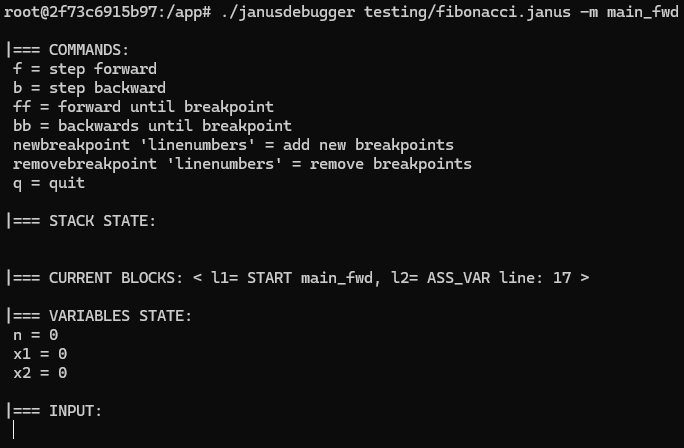
\includegraphics[width=1\textwidth]{pictures/fib_opening.png}
    \label{fig:fib_open}
\end{figure}

Non avendo inserito nessun breakpoint, proviamo ad avanzare fino alla fine del programma con "ff", il risultato dovrebbe essere x1 = 5 e x2 = 8:
\begin{figure}[!h]
    \centering
    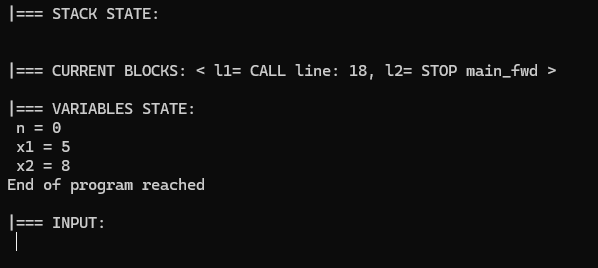
\includegraphics[width=1\textwidth]{pictures/fib_1.png}
    \label{fig:fib1}
\end{figure}

Adesso inseriamo due breakpoint a riga 7 dove c'è l'istruzione "x1 += 1" e a riga 12 dove c'è l'istruzione "x1 += x2" tramite il comando "newbreakpoint 7 12", la prima viene eseguita una volta soltanto quando n è uguale a 0 mentre la seconda viene eseguita dopo ogni chiamata a fib dove n != 0, procediamo eseguendo il comando "bb":
\begin{figure}[!h]
    \centering
    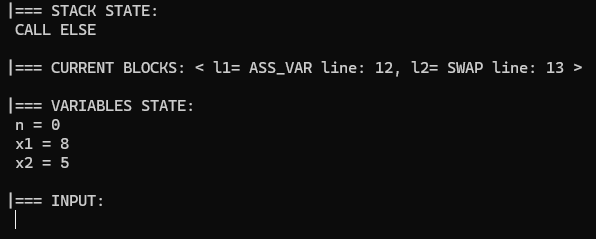
\includegraphics[width=1\textwidth]{pictures/fib_2cut.png}
    \label{fig:fib2}
\end{figure}

Adesso possiamo notare alcune differenze. Visto che ci siamo mossi in direzione backward il primo blocco \emph{l1} è quello che contiene l'istruzione indicata dal breakpoint che deve ancora essere eseguita, mentre il secondo blocco \emph{l2} contiene l'istruzione appena eseguita, questa è uno swap (x1 $<=>$ x2) quindi i valori di x1 e x2 sono invertiti. Inoltre è ora possibile vedere due blocchi all'interno dello stack: la call della procedura fib e il ramo else dell'if all'interno del quale si trova l'istruzione cercata.
\bigskip

Visto che questo breakpoint viene incontrato ad ogni chiamata di fib in cui n!=0, e lo stack del nostro programma ne contiene più di una proviamo a rimuoverlo dai breakpoint tramite il comando "removebreakpoint 12", poi eseguiamo nuovamente il comando "bb" per raggiungere l'altro breakpoint:
\begin{figure}[!h]
    \centering
    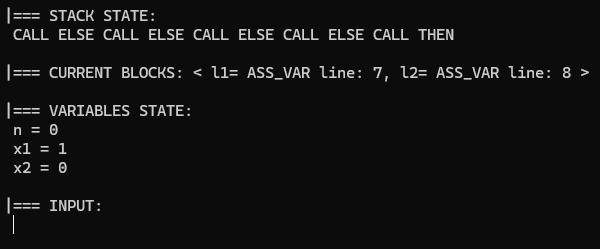
\includegraphics[width=1\textwidth]{pictures/fib_3cut.png}
    \label{fig:fib3}
\end{figure}

Ora ci troviamo all'inizio della serie di fibonacci, è possibile vedere tutte le chiamate a fib che il programma effettua all'interno dello stack sulla cui cima è presente un elemento di tipo \emph{THEN} a cui ci troviamo perchè la condizione n=0 è soddisfatta in questo punto. L'istruzione successiva al nostro breakpoint (in direzione forward) è l'assegnamento x2+=1, proviamo quindi ad eseguire il comando "f":
\begin{figure}[!h]
    \centering
    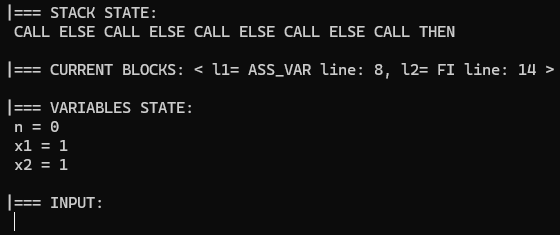
\includegraphics[width=1\textwidth]{pictures/fib_4cut.png}
    \label{fig:fib4}
\end{figure}

Com'è possibile vedere, abbiamo avanzato di una istruzione, l'assegnamento x2+=1 si trova ora nella posizione \emph{l1} che, avendo fatto un passo forward, indica l'istruzione appena eseguita.
\bigskip

Facciamo anche un tentativo di inserire un comando non esistente come "test" e vediamo che il debugger ci dà un messaggio di errore senza interrompere l'esecuzione, possiamo infatti continuare ad inserire altri comandi:
\begin{figure}[!h]
    \centering
    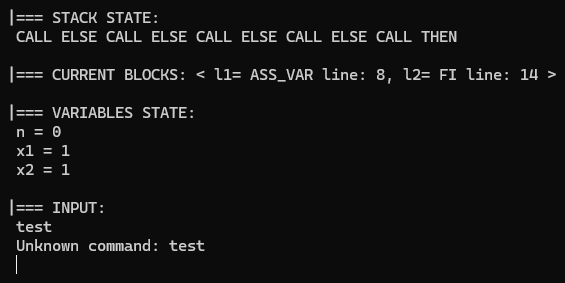
\includegraphics[width=1\textwidth]{pictures/fib_5cut.png}
    \label{fig:fib5}
\end{figure}


\section{Installazione requisiti}

Gli unici requisiti del progetto sono rappresentati da un compilatore per C++, noi abbiamo usato g++, e dal tool e runtime di ANTLR. Il tool è il generatore vero e proprio del lexer e del parser nel linguaggio desiderato, mentre il runtime è l'insieme delle librerie necessarie per il funzionamento corretto. Per l'installazione del tool e del runtime di ANTLR invitiamo a far riferimento al sito ufficiale~\cite{antlrwebsite}, ma di seguito andremo a spiegare a puro scopo informativo come abbiamo fatto noi, all'interno di un container docker con sistema operativo Ubuntu utilizzato come ambiente di sviluppo, e come eseguire il progetto.
Per installare i tool da barra di comando è necessario il gestore di pacchetti pip, quindi abbiamo utilizzato il comando:\smallskip

\noindent apt update \&\& apt install python3-pip build-essential libantlr4-runtime-dev\smallskip

\noindent per installare rispettivamente: pip, g++ e il runtime di ANTLR. Per installare, invece, il tool di ANTLR abbiamo poi usato il comando:\smallskip

\noindent pip install antlr4-tools\smallskip

Bisogna assicurarsi inoltre che la versione del tool e la versione del runtime siano la stessa, nel nostro caso la versione utilizzata è la 4.10. Per specificare con che versione del tool generare i file, possiamo usare il comando:\smallskip

\noindent export ANTLR4\_TOOLS\_ANTLR\_VERSION=4.10\smallskip

Ora possiamo andare ad utilizzare ANTLR per generare il lexer e il parser per la nostra grammatica janus.g4 tramite il comando:\smallskip

\noindent antlr4 -Dlanguage=Cpp -visitor janus.g4\smallskip

Grazie al parametro "-Dlanguage" possiamo specificare il linguaggio di programmazione in cui generare i nostri file, nel nostro caso cpp, e tramite il parametro "-visitor" ci assicuriamo che vengano creati i file del visitor, una classe che permette di visitare l'albero di parsing, e di cui andremo a creare un figlio personalizzato per la costruzione del CFG all'interno del file CFGbuilder.h.

Infine possiamo compilare ed eseguire il nostro progetto, andando ad includere i file necessari generati da ANTLR, il runtime e il nostro main. Usiamo quindi i comandi:\smallskip

\noindent g++ -std=c++20 -I janus -I /usr/include/antlr4-runtime main.cpp janus/janus*.cpp -lantlr4-runtime -o janusdebugger\smallskip

\noindent ./janusdebugger myprogram.janus\smallskip

Specifichiamo che i file generati da ANTLR sono locati all'interno della cartella "janus", che la versione utilizzata di C++ è la 20, e il codice non é compatibile con versioni precedenti.

\newpage
\section{Implementazione}

Il primo passo per l'implementazione è stato definire la grammatica nel formato ".g4" richiesto da ANTLR. Di seguito la grammatica combinata \emph{janus.g4} effettivamente utilizzata nel progetto come sorgente per ANTLR in modo da creare lexer e parser:

\begin{figure}[!h]
\small
\centering
\hspace*{-0.5cm}
$\begin{array}{r@{\quad}c@{\quad}l}
\text{grammar} & \text{janus;} \\[0.5em]
\text{program} & ::= & \text{variables}? \text{ functions;} \\
\text{variables} & ::= & \text{variableName ( '[' Digit ']' )?} \mid \text{variables variables;} \\
\text{functions} & ::= & \text{function} \mid \text{function functions;} \\
\text{function} & ::= & \text{'procedure'} \text{ functionName statements}?; \\
\text{statements} & ::= & \text{assignmentExpression} \mid \text{ifConstructor} \mid \text{loopConstructor} \\
& & \mid \text{functionCall} \mid \text{skip} \mid \text{statements statements;} \\
\text{assignmentExpression} & ::= & \text{variableName ( '[' expression ']' )? assignmentOperator expression;} \\
\text{ifConstructor} & ::= & \text{ifExpression fiExpression} \mid \\ & & \text{ifExpression elseExpression fiExpression;} \\
\text{ifExpression} & ::= & \text{'if' '('? expression ')'? 'then' statements;} \\
\text{elseExpression} & ::= & \text{'else' statements;} \\
\text{fiExpression} & ::= & \text{'fi' expression;} \\
\text{loopConstructor} & ::= & \text{fromExp doExp}? \text{ loopExp}? \text{ untilExp;} \\
\text{fromExp} & ::= & \text{'from' expression;} \\
\text{untilExp} & ::= & \text{'until' expression;} \\
\text{doExp} & ::= & \text{'do' statements;} \\
\text{loopExp} & ::= & \text{'loop' statements;} \\
\text{expression} & ::= & \text{Digit} \mid \text{TextDigit ( '[' expression ']' )?} \mid \\ & & \text{expression operator expression} \mid \text{'(' expression ')';}\\
\text{functionCall} & ::= & \text{call} \text{ functionName;} \\
\text{skip} & ::= & \text{'skip';} \\
\text{assignmentOperator} & ::= & \text{'+='} \mid \text{'-='} \mid \text{'\textless=\textgreater'} \mid \text{'\^{}= '}; \\
\text{relationalOperator} & ::= & \text{'='} \mid \text{'!='} \mid \text{'\textless'} \mid \text{'\textgreater'} \mid \text{'\textless='} \mid \text{'\textgreater='}; \\
\text{arithmeticOperator} & ::= & \text{'*'} \mid \text{'+'} \mid \text{'-'} \mid \text{'/'} \mid \text{'\%'}; \\
\text{bitwiseOperator} & ::= & \text{'\&'} \mid \text{'\textbar'} \mid \text{'\^{}'}; \\
\text{logicalOperator} & ::= & \text{'\&\&'} \mid \text{'\textbar\textbar'}; \\
\text{operator} & ::= & \text{arithmeticOperator} \mid \text{bitwiseOperator} \mid \\ & & \text{relationalOperator} \mid \text{logicalOperator}; \\
\text{call} & ::= & \text{'call'} \mid \text{'uncall'}; \\
\end{array}$
\caption{Grammatica Janus utilizzata per il debugger}
\label{fig:janus_grammar}
\end{figure}


Il codice del debugger step-by-step in C++ è diviso in quattro file spiegati nel dettaglio nelle seguenti sottosezioni. Main.cpp è il file che contiene il main, structures.h contiene le definizioni delle strutture utilizzate, come il CFG, CFGbuilder.h contiene la classe figlio del visitor di ANTLR, scorre l'albero di parsing per costruire il CFG, mentre ReversibleJanusInterpreter.h contiene la classe principale che applica la semantica reversibile illustrata precedentemente.

\subsection{main.cpp}
Subito, il file main.cpp gestisce l'input del debugger da riga di comando, esegue un controllo se è in grado di aprire il file e legge i parametri -m e -d se inseriti dall'utente, procede poi con l'inizializzazione del lexer e del parser generati da ANTLR, e l'inizializzazione del nostro CFGbuilder che costruisce il CFG a partire dall'albero di parsing generato dal parser. Qui è anche presente la logica per trovare la procedura main all'interno del CFG creato dal CFGbuilder e i due label inziali della procedura. Poi viene inizializzato il nostro ReversibleJanusInterpreter che richiede il CFG e i due label di partenza come parametri.

Infine il main.cpp gestisce gli input dell'utente a tempo di esecuzione, l'utente puo infatti inserire "f" (forward) o "b" (backward), rispettivamente per eseguire un passo in avanti o indietro nell'esecuzione, oppure, "ff" o "bb" rispettivamente per mandare avanti o indietro l'esecuzione fino al prossimo breakpoint, chiaramente se non sono stati inseriti breakpoint, l'esecuzione procede fino alla fine o fino all'inizio del programma, una volta raggiunto uno di questi due punti è stampato a video un messaggio per farlo capire all'utente (rispettivamente: "End of program reached" oppure "Start of program reached"). L'esecuzione non termina raggiungendo uno dei due estremi, è infatti possibile continuare la navigazione del debugger finchè non si inserisce "q" (quit) come input da tastiera.


\subsection{Le strutture del debugger}
Nel file structures.h sono definite le strutture utilizzate nel nostro codice, in particolare sono definiti gli elementi dello stack $\pi$, i blocchi delle singole operazioni e il control-flow graph. Il tipo "Label" è definito come un semplice size\_t (tipo unsigned che comprende numeri interi maggiori o uguali a zero) che abbiamo rinominato per motivi di chiarezza e coerenza con la semantica reversibile.

\begin{figure}[h]
    \centering
    \begin{minipage}{0.95\textwidth}
        \ttfamily 
        struct Block \hspace*{10em} struct StackItem\\
        \{ \hspace*{15.5em} \{ \\
        \hspace*{1em} Label label; \hspace*{9.5em} StackItemType type; \\
        \hspace*{1em} BlockType type; \hspace*{8em} Label l; \\
        \hspace*{1em} Label line; \hspace*{9em} \}; \\
        \\
        \hspace*{1em} string varName; \\
        \hspace*{1em} AssignmentOp op;\\
        \hspace*{1em} janusParser::ExpressionContext *expr1 = nullptr; \\
        \hspace*{1em} janusParser::ExpressionContext *expr2 = nullptr; \\
        \hspace*{1em} string procedurename; \\
        \hspace*{1em} janusParser::ExpressionContext *condExpr = nullptr;\\
        \}; \\
    \end{minipage}
    \caption{struttura del blocco di un'operazione e di un elemento dello stack nel debugger}
    \label{fig:block}
\end{figure}

Come mostrato in Figura~\ref{fig:block} ogni blocco è composto da tre campi necessari per la sua inizializzazione, il label del blocco, la riga di codice a cui si trova il blocco (line) e il tipo (BlockType type) del blocco che può essere uno tra i seguenti: START, STOP, ASS\_VAR, ASS\_ARR, SWAP, SKIP, CALL, UNCALL, IF, FI, FROM, UNTIL. Ci sono inoltre altri sei campi utilizzati a seconda del tipo del nostro blocco.

I primi quattro campi sono inizializzati nei blocchi degli assegnamenti e nei blocchi di swap, "varName" e "op" contengono rispettivamente il nome della variabile che viene alterata e l'operazione eseguita. Per quanto riguarda "expr1" ed "expr2", questi campi contengono degli \emph{ExpressionContext}, strutture dati fornite da ANTLR che compongono i nodi dell'albero di parsing, il loro contenuto dipende dal tipo di assegnamento, se è infatti quello di una variabile expr1 contiene l'ExpressionContext di cio che si trova alla destra dell'operando ed expr2 rimane vuoto, nel caso in cui l'assegnamento sia quello di un array, expr1 contiene l'ExpressionContext di ciò che si trova tra le parentesi quadre "[]" ed expr2 contiene l'ExpressionContext di cio che si trova alla destra dell'operando. La valutazione del contenuto dei context verrà fatta successivamente all'interno della classe "ReversibleJanusInterpreter" nel file "ReversibleJanusInterpreter.h". Gli ultimi due campi sono usati rispettivamente, "procedurename" quando il blocco è quello di una procedure call/uncall e contiene il nome della procedura chiamata, mentre "condExpr" quando nel blocco è presente una condizione (quindi if, fi, from e until) e contiene l'ExpressionContext della condizione. Vogliamo far notare che grazie a questa struttura dei blocchi il debugger non implementa direttamente la funzione \emph{context} presentata nella semantica~\ref{sec:LV26}, infatti questa veniva utilizzata una volta incontrata una condizione per capire se fa parte di un condizionale o un loop, questo non è necessario perchè esiste il campo che indica il tipo del blocco (BlockType \emph{type}) e dal tipo di blocco è possibile capire di che costrutto fa parte.
\bigskip

Gli elementi dello stack, invece, sono definiti da un tipo (StackItemType type) che può essere, come indicato nella semantica, uno tra i seguenti: CALL, UNCALL, IF\_TRUE, IF\_FALSE, LOOP1, LOOP2. Ogni elemento dello stack è definito, inoltre, da un label (Label l) questo indica un blocco che è necessario tenere da parte per il funzionamento del debugger e che dipende dal tipo dell'elemento nello stack. Per gli elementi di tipo CALL e UNCALL il label è quello del blocco della chiamata (utilizziamo il termine "chiamata" anche per le uncall in quanto, come illustrato nella semantica reversibile, queste sono procedure con un proprio cfg indipendente da quello delle procedure da cui sono state create per inversione), per gli elementi di tipo IF\_TRUE e IF\_FALSE, il label inserito nello stack è quello del test (la condizione iniziale), essenziale per assicurare la reversibilità del debugger,  e per gli elementi di tipo LOOP1 e LOOP2, il label inserito è quello rispettivamente dei blocchi FROM e UNTIL (che contengono le condizioni del ciclo: assertion e test).

Vogliamo far notare ora una piccola differenza tra la semantica reversibile illustrata nella sezione~\ref{sec:LV26}~\cite{LV26} e la nostra implementazione del debugger, nella semantica infatti gli elementi dello stack possono avere piu di un label inserito. Nel caso degli IF\_TRUE e degli IF\_FALSE vengono inseriti entrambi i label delle condizioni, e nel caso di LOOP1 e LOOP2 vengono inseriti, non solo i label di entrambe le condizioni, ma anche gli statement dei due path del ciclo. Nell'implementazione presentata abbiamo considerato ciò non necessario e abbiamo deciso di evitarlo, ottenendo una soluzione del tutto equivalente, in quanto avevamo la possibilità di reperire queste informazioni in altro modo grazie alla nostra costruzione delle strutture dati. Infatti, nel caso degli IF, quando ci troviamo a rimuovere l'elemento dallo stack (IF\_TRUE o IF\_FALSE) l'elemento indicato dal nostro label corrente l2 è proprio il blocco contenente la seconda condizione, pertanto è futile inserirla nello stack, ci basta inserire la prima e confrontarla con quella nel blocco l2 che stiamo valutando, la nostra struttura del cfg~\ref{fig:programcfg} ci permette a tale scopo, attraverso la mappa "blocks", di ottenere un blocco a partire dalla sua label (discorso equivalente nel caso backward ma con l1). Nel caso dei LOOP, si applica lo stesso discorso per le condizioni, ma nella semantica reversibile al contrario della nostra implementazione, gli elementi dello stack contengono anche i blocchi di statements dei due path del loop, anche questi sono futili nel nostro caso perchè utilizzati in combinazione con la funzione entry() per trovare il primo blocco degli statement e capire in che direzione procedere, ma nella nostra implementazione le mappe "forwardFlow" e "backwardFlow" associano ad ogni label tutte le possibili label successive (e precedenti), di solito la label successiva è singola ma nei casi dei blocchi associati alla seconda condizione del ciclo le label successive sono due e l'implementazione decide se prendere la prima o la seconda in base al risultato della condizione (discorso analogo nel caso backwards), pertanto non serve salvare all'interno dello stack i blocchi di statement del ciclo. E' per queste ragioni che le funzioni entry() ed exit() non sono direttamente implementate nel nostro debugger.
\bigskip

\begin{figure}[h]
    \centering
    \begin{minipage}{0.95\textwidth}
        \ttfamily 
        struct ProgramCFG \\
        \{ \hspace*{15.5em} \\
        \hspace*{1em} map<string, int> variables; \\
        \hspace*{1em} map<string, vector<int>> arrays;\\
        \\
        \hspace*{1em} map<Label, Block> blocks;\\
        \hspace*{1em} map<Label, vector<Label>> forwardFlow; \\
        \hspace*{1em} map<Label, vector<Label>> backwardFlow;\\
        \\
        \hspace*{1em} map<string, Label> procedureEntry;\\
        \hspace*{1em} map<string, Label> procedureExit; \\
        \\
        \hspace*{1em} map<string, Label> reverseprocedureEntry; \\
        \hspace*{1em} map<string, Label> reverseprocedureExit;\\
        \\
        \hspace*{1em} void addEdge(Label u, Label v) \\
        \hspace*{1em} \{ \\
        \hspace*{2em} forwardFlow[u].push\_back(v); \\
        \hspace*{2em} backwardFlow[v].push\_back(u); \\
        \hspace*{1em} \} \\
        \}; \\
    \end{minipage}
    \caption{struttura dati del Control Flow Graph}
    \label{fig:programcfg}
\end{figure}

L'ultima struttura dati definita nel file structures.h è quella del Control Flow Graph, illustrata in Figura~\ref{fig:programcfg}. Per questa implementazione sono state utilizzate le mappe (map), insiemi ordinati di coppie chiave-valore. Anche se non era specificato nella semantica, abbiamo deciso di includere lo store $\sigma$ delle variabili e degli array all'interno della struttura del cfg (rispettivamente all'interno delle mappe variables e arrays), in modo che un'istanza di questa possa effettivamente rappresentare un programma in maniera completa. Dopo ciò, all'interno della struttura abbiamo inserito una mappa di blocchi (blocks) che contiene tutti i blocchi del programma, e le due mappe "forwardFlow" e "backwardFlow" che contengono per ogni blocco i suoi possibili successori, rispettivamente in avanti e indietro (sotto forma di Label) ed implementano la funzione "flow" della semantica reversibile, illustrata in Figura~\ref{fig:cfg}. Ci sono anche mappe per il salvataggio di tutte le entry (Label di inizio: START) ed exit (ultimo Label: STOP) delle procedure, sia per la versione forward (procedureEntry e procedureExit) sia per la versione backward (reverseprocedureEntry, reverseprocedureExit). Lo stesso nome di procedura cercato come chiave all'interno di procedureEntry e reverseprocedureExit risulta rispettivamente nel label di start del cfg della procedura forward e nel label stop del cfg della procedura backward, entrambi contenenti la stessa operazione sebbene siano blocchi diversi. La struttura termina con la funzione "addEdge" che serve a creare un collegamento bidirezionale tra due blocchi, la funzione infatti aggiunge il secondo blocco al forwardFlow del primo, e il primo al backwardFlow del secondo. AddEdge è utilizzata all'interno del CFGbuiler, nel file "CFGbuilder.h" per creare gli effettivi collegamenti del cfg che diventa, quindi, una struttura in cui a partire da un qualsiasi blocco è possibile avanzare ed indietreggiare step-by-step verso tutti gli altri blocchi collegati, e a partire dal nome di una procedura è possibile accedere ai cfg forward e backward dedicati da entrambi i loro estremi (start e stop).

\subsection{Dall'albero di parsing al Control-Flow Graph}
La classe CFGbuilder definita nel file "CFGbuilder.h" rappresenta il vero e proprio punto di contatto tra gli strumenti forniti da ANTLR e il codice del nostro debugger. Infatti questa classe eredita dalla classe \emph{BaseVisitor} che permette di scorrere l'albero di parsing generato da ANTLR attraverso il metodo "visit" che svolge una visita di tipo DFS (depth-first search). I nodi di quest'albero sono creati dal parser in base alle regole della grammatica janus.g4 presentata in Figura~\ref{fig:janus_grammar}. La classe BaseVisitor (tramite il metodo visit) esegue un metodo diverso per ogni tipologia di nodo dell'albero, questi metodi sono chiamati con "visit" seguito dal tipo di nodo (nome della regola nella grammatica). Il visitor base si limita a scorrere l'albero chiamando le visit sui children, ma, nella nostra classe CFGbuilder i metodi sono sovrascritti (overriding) in modo da eseguire specifiche funzioni spiegate a breve. Quindi, é proprio mentre visitiamo l'albero di parsing che questi metodi generano la struttura essenziale del nostro debugger, il Control-Flow Graph.\bigskip

\begin{figure}[h]
    \centering
    \hspace*{-1.5cm}
    \begin{minipage}{1.5\textwidth}
        \ttfamily 
        class CFGBuilder : public janusBaseVisitor \\
        \{\\
        private:\\
        \hspace*{1em} ProgramCFG cfg;\\
        \hspace*{1em} Label nextLabel = 1;\\
        \hspace*{1em} Label createLabel()\\
        \hspace*{1em} \{\\
        \hspace*{1em} return nextLabel++;\\
        \hspace*{1em} \}\\
        \\
        public:\\
        \hspace*{1em} ProgramCFG getCFG() \{ return cfg; \}\\
        \hspace*{1em} virtual any visitVariables(janusParser::VariablesContext *ctx) override \\
        \hspace*{1em} virtual any visitFunction(janusParser::FunctionContext *ctx) override\\
        \hspace*{1em} virtual any visitStatements(janusParser::StatementsContext *ctx) override\\
        \hspace*{1em} virtual any visitAssignmentExpression(janusParser::AssignmentExpressionContext \\ \hspace*{4em} *ctx) override \\
        \hspace*{1em} virtual any visitIfConstructor(janusParser::IfConstructorContext *ctx) override \\
        \hspace*{1em} virtual any visitLoopConstructor(janusParser::LoopConstructorContext *ctx) override\\
        \hspace*{1em} virtual any visitFunctionCall(janusParser::FunctionCallContext *ctx) override \\
        \hspace*{1em} virtual any visitSkip(janusParser::SkipContext *ctx) override\\
        \}; \\
    \end{minipage}
    \caption{classe CFGbuilder (senza le implementazioni dei metodi)}
    \label{fig:cfgbuilder}
\end{figure}

\begin{figure}[t]
    \centering
    %\hspace*{4.5cm}
    \begin{minipage}{1\textwidth}
        \ttfamily 
        a b c \\
        \\
        procedure main\\
        \hspace*{1em} if a = 0 then\\
        \hspace*{2em} b += 1\\
        \hspace*{2em} c <=> b\\
        \hspace*{1em} fi a = 0\\
    \end{minipage}
    \caption{Programma esempio}
    \label{fig:programcfg}
\end{figure}

\begin{figure}[!h]
    \centering
    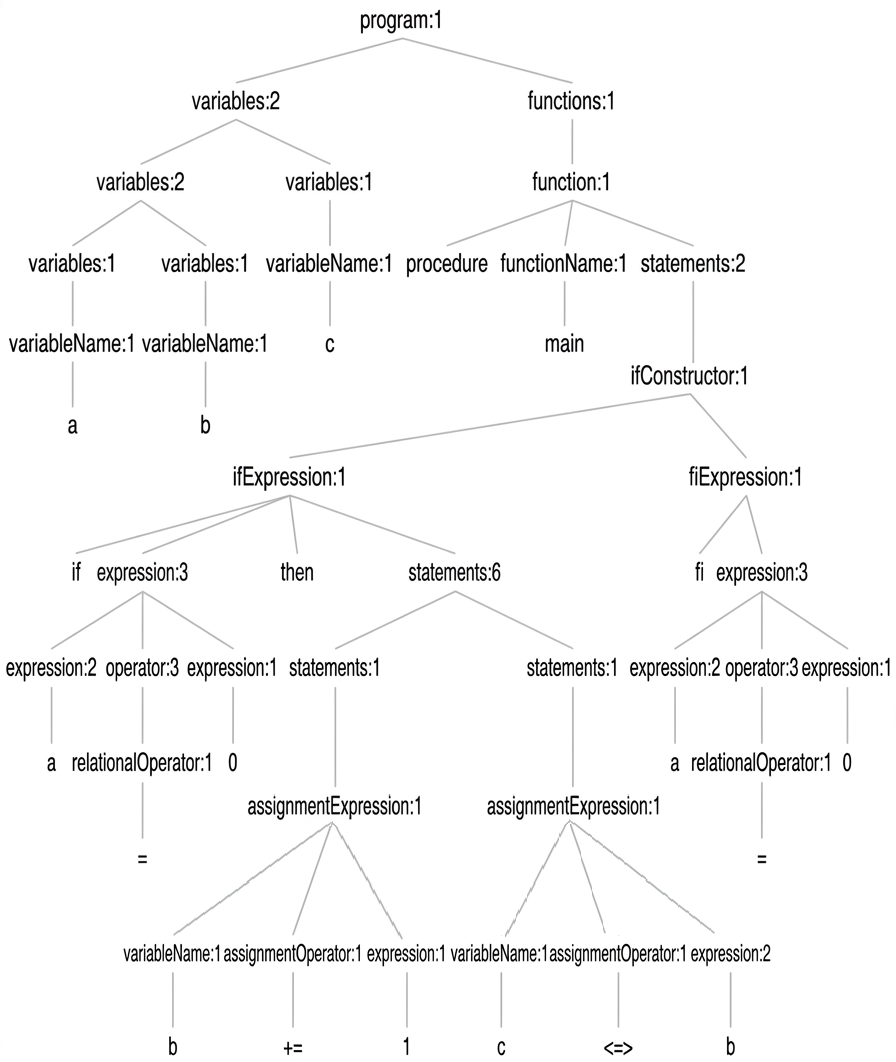
\includegraphics[width=0.89\textwidth]{pictures/parsetree3.png}
    \caption{Albero di parsing del programma esempio}
    \label{fig:parsetree}
\end{figure}
\bigskip

Di seguito andiamo a spiegare cosa succede quando ciascuno dei metodi viene chiamato durante la visita dell'albero di parsing, nel nome del metodo è inserito il tipo di nodo che viene visitato per eseguirlo.
\begin{itemize}
\item Il metodo "\emph{visitVariables}" inizializza variabili ed array all'interno del cfg. 
\item Il metodo "\emph{visitFunction}" crea i blocchi start e stop per entrambe le direzioni della procedura, ovvero forward e backward, se sono presenti degli statement all'interno della procedura, dopo aver eseguito la visit di questi, unisce i blocchi estremi del cfg degli statement interni con lo start e lo stop.
\item Il metodo "\emph{visitStatements}" gestisce gli statement in sequenza, chiama la visit dei sotto-statement e poi unisce gli estremi dei loro cfg in maniera sequenziale.
\item Il metodo "\emph{visitAssignmentExpression}" crea il blocco dell'assegnamento tenendo presente l'operatore per assegnare la corretta "AssignmentOp" (tipo di operatore) al blocco, poi crea il blocco inverso.
\item Il metodo "\emph{visitIfConstructor}" crea i blocchi if e fi inserendo le condizioni associate a ciascuno, e i corrispettivi blocchi if e fi backwards con le condizioni invertite tra loro. Poi chiama una visit degli statements all'interno del then e costruisce il cfg dell'if collegando i blocchi degli statements con quelli creati, se è presente anche un else la procedura si ripete allo stesso modo per l'altro ramo, altrimenti vengono collegati i due blocchi if e fi.
\item Il metodo "\emph{visitLoopConstructor}" crea i blocchi from e until inserendo le condizioni associate a ciascuno, e i corrispettivi blocchi from e until backwards con le condizioni invertite tra loro. Poi, se presenti, chiama le visit sugli statement all'interno delle sezioni do e loop, e costruisce il cfg del loop collegando i blocchi degli statement di queste sezioni con quelli creati.
\item Il metodo "\emph{visitFunctionCall}" crea il blocco della chiamata tenendo in considerazione il tipo della chiamata (call oppure uncall) e il nome della procedura, poi crea il blocco backward invertendo il tipo.
\item Il metodo "\emph{visitSkip}" crea due blocchi di tipo skip, uno per il cfg forward e uno per il cfg backward.
\end{itemize}
E' importante far notare che visitAssignmentExpression, visitIfConstructor, visitLoopConstructor, visitFunctionCall e visitSkip hanno come valori di ritorno delle tuple di quattro elementi, rispettivamente i label degli estremi del pezzo di cfg che hanno costruito per le due versioni forward e backward. Infatti questi metodi sono chiamati da visitStatements che ricostruisce la catena di blocchi e la restituisce (sempre mediante una tupla di estremi) a visitFunction che le associa i blocchi start e stop.

\subsection{Implementazione delle regole della semantica reversibile}
La classe ReversibleJanusInterpreter all'interno del file "ReversibleJanusInterpreter.h" è il punto dove viene implementata la vera logica del debugger. A partire dal cfg e dai due label iniziali (parametri di inizializzazione della classe attraverso il costruttore) questa classe fornisce tutti gli strumenti per avanzare step-by-step in avanti (metodo "stepForward") e indietro (metodo "stepBackward") durante l'esecuzione del nostro programma.\bigskip

\begin{figure}[h]
    \centering
    \begin{minipage}{1.2\textwidth}
        \ttfamily 
        class ReversibleJanusInterpreter\\
        \{\\
        public:\\
        \hspace*{1em} ProgramCFG cfg;\\
        \hspace*{1em} Label l1 = 0;\\
        \hspace*{1em} Label l2 = 0;\\
        \hspace*{1em} vector<StackItem> pi;\\
        \\
        \hspace*{1em} ReversibleJanusInterpreter(ProgramCFG pCFG, Label startL1, Label startL2) :\\
        \hspace*{1em} cfg(move(pCFG)), l1(startL1), l2(startL2) {}\\
        \\
        \hspace*{1em} int evalExpr(janusParser::ExpressionContext *ctx)\\
        \hspace*{1em} void applyOp(string var, AssignmentOp op, int val, int idx = -1)\\
        \hspace*{1em} AssignmentOp invertOp(AssignmentOp op)\\
        \hspace*{1em} bool stepForward()\\
        \hspace*{1em} bool stepBackward()\\
        \hspace*{1em} void printState(string m="") \\
        \}; \\
    \end{minipage}
    \caption{classe ReversibleJanusInterpreter (senza le implementazioni dei metodi)}
    \label{fig:reversiblejanusinterpreter}
\end{figure}

I primi tre metodi sono di supporto per i metodi stepForward e stepBackward:
\begin{itemize}
\item Il metodo \emph{evalExpr} prende come parametro un ExpressionContext (nodo dell'albero di parsing) e lo valuta per restituire un valore intero. Come mostrato dalla grammatica in Figura~\ref{fig:janus_grammar}, una expression può avere come valore un numero intero, un nome di variabile o di array con relativo indice, oppure due expression unite da un operatore. Questo metodo analizza il contenuto del context fornito, e di conseguenza calcola i valori delle operazioni e valuta le condizioni, che possono avere come valori di ritorno 1 o 0 (true e false).
\item Il metodo \emph{applyOp} esegue le operazioni di addizione, sottrazione e xor delle AssignmentExpressions (non si occupa, però, delle operazioni di swap) aggiornando il cfg. I suoi parametri rappresentano il nome della variabile (o array), il tipo di operazione eseguita, il valore con cui eseguire l'operazione e il parametro facoltativo dell'indice nel caso degli array.
\item Il metodo \emph{invertOp} prende come parametro l'operazione di un AssignmentExpression e la inverte, utile nello stepBackward per eseguire l'inverso delle operazioni, implementa le regole di inversione degli assegnamenti illustrate in Figura~\ref{fig:inverter}.
\end{itemize}

I metodi \emph{stepForward} e \emph{stepBackward} eseguono rispettivamente uno step in avanti e indietro nel nostro cfg (fanno avanzare o indietreggiare l'esecuzione di un passo). Il funzionamento si basa su uno switch col valore del tipo del blocco indicato dal secondo label \emph{l2} per il caso forward e \emph{l1} per il caso backward (label che indica la prossima operazione da eseguire, partendo dall'inizio di un programma l2 rappresenta la prima operazione in quanto il blocco l1 contiene lo start), a seconda quindi del BlockType, viene eseguita la corrispondente implementazione delle regole mostrate nelle Figure~\ref{fig:reversible-smallstep} e~\ref{fig:reversible-ifloop} e nelle Figure~\ref{fig:reversible-smallstep-backward} e~\ref{fig:reversible-ifloop-backward}. Facciamo notare che non abbiamo implementato direttamente le funzioni entry ed exit presentate in Figura~\ref{fig:entryexit} ma che la semantica è del tutto equivalente grazie alla nostra costruzione della struttura del Control-Flow Graph, infatti le entry e le exit delle procedure sono salvate all'interno del cfg, mentre le entry e le exit degli altri statement sono reperibili semplicemente con un passo in avanti o indietro, quando sono possibili piu strade (come nel caso di un if) l'opzione dedicata del nostro switch gestisce quale strada prendere. Anche la funzione \emph{ctx()} non è stata implementata direttamente, il suo ruolo è svolto dal controllo del BlockType corrente. La nostra implementazione include inoltre, la regola SWAP anche se non è presentata all'interno della semantica reversibile.\smallskip

Il metodo \emph{printState} è chiamato dal main ad ogni passo (o al raggiungimento di un breakpoint o di un estremo del programma) e serve a mostrare a video lo stato attuale delle variabili e degli array, inoltre stampa sulla console il blocco appena eseguito e il prossimo blocco da eseguire (l'ordine dipende dalla direzione dell'ultimo passo, se è appena stato eseguito uno step forward viene mostrato prima il blocco appena eseguito e poi il prossimo blocco da eseguire, se invece è appena stato eseguito uno step backward l'ordine è invertito) e lo stato dello stack nel momento della chiamata.

\section{Conclusioni e possibili lavori futuri}

Costruire un debugger reversibile per un linguaggio intrinsecamente reversibile come Janus è concettualmente molto diverso rispetto a farlo per un linguaggio non reversibile. Il vantaggio fondamentale è che in un linguaggio reversibile l'inversione è una proprietà semantica del linguaggio stesso, mentre in un linguaggio non reversibile va artificialmente ricostruita o simulata dal debugger. Un debugger per un linguaggio tradizionale richiederebbe un sistema per salvare in memoria i cambiamenti fatti allo stato della computazione ad ogni passo, altrimenti operazioni di sovrascrittura come gli assegnamenti non potrebbero essere rese reversibili in quanto prevedono che alcune informazioni siano scartate. Il problema degli assegnamenti è risolto in Janus grazie al sistema di trasformazioni reversibili delle variabili senza che il valore di queste venga scartato (ad esempio incrementando o decrementando). Anche i condizionali e i cicli richiederebbero di salvare il risultato della condizione nel primo caso e il numero di iterazioni nel secondo.
\medskip

Con questo documento è stato introdotto un debugger step-by-step per il linguaggio di programmazione reversibile Janus che permette all'utente di muoversi in avanti e indietro nella computazione a singoli passi tra i blocchi del programma oppure tra breapoint diversi e analizzare lo stato delle variabili e degli array e lo stato della configurazione tramite i blocchi correnti e lo stack, in ogni punto del programma. Sono stati forniti, inoltre, i dettagli della semantica utilizzata e dell'implementazione della stessa con le relative scelte strutturali e le differenze ove presenti, in modo da poter fornire tutti gli strumenti per lavorare sul codice ed arricchirlo o adattarlo a specifiche esigenze.
\medskip

Tuttavia il progetto si limita ai costrutti base di Janus, un possibile aggiornamento futuro può essere l'aggiunta di nuovi costrutti o nuove funzionalità per il linguaggio, altri interpreti per janus permettono gia, ad esempio, l'inizializzazione di variabili locali. Anche l'aggiunta di breakpoint che si attivano solo nel caso in cui certe condizioni vengono rispettate potrebbe essere un aggiunta utile. Sebbene altri interpreti permettono la generazione dell'inverso del codice, nel nostro caso non è strettamente necessario in quanto il debugger è reversibile da sè, quindi basta partire dal fondo del programma e procedere all'indietro per ottenere l'inverso, tuttavia può tornare utile inserire un generatore di codice in altri linguaggi come Java o C++. Un altro lavoro che potrebbe tornare utile ad un utente che desidera fare debugging anche di codice di grandi dimensioni potrebbe essere l'inserimento di un'nterfaccia grafica, magari con la visualizzazione a schermo del codice per intero evidenziando la riga attualmente in esecuzione. Un ultimo aggiornamento che potrebbe essere fatto è la possibilità di cambiare il valore di un assegnamento durante l'esecuzione del debugger per poter fare test sugli esiti diversi che il programma può ottenere senza dover riscrivere il codice e rieseguire il debugger. Questo debugger fa uso di ANTLR per generare il lexer ed il parser, uno sviluppo futuro può essere la scrittura di questi senza partire da un generatore, in modo da ridurre le dipendenze da installare ed evitare eventuali bug relativi ad aggiornamenti di queste.

\bibliographystyle{plain}
\bibliography{bibliography}
\end{document}